\documentclass[tid,table]{texufpel} %use tid para doutorado e ti para mestrado



\usepackage{enumerate}
\usepackage[utf8]{inputenc} % acentuacao
\usepackage{graphicx} % para inserir figuras
\usepackage{url}

\hypersetup{
    hidelinks, % Remove coloração e caixas
    unicode=true,   %Permite acentuação no bookmark
    linktoc=all %Habilita link no nome e página do sumário
}

\usepackage{xcolor}
\usepackage{tabularx}
\usepackage{tablefootnote}

\usepackage{pdflscape}
\usepackage{afterpage}
\usepackage{capt-of}% or use the larger `caption` package

\usepackage[color=green!40]{todonotes}
\newcommand {\AY} {\todo[inline, color=green]} %comentarios Adenauer
\newcommand {\AP} {\todo[inline, color=yellow]} %Comentarios Ana

\unidade{Centro de Desenvolvimento Tecnológico}
\programa{Programa de Pós-Graduação em Computação}
\curso{Ciência da Computação}


\title{Avaliação de Estratégias de Segurança Adaptativa para a Internet das Coisas}


% VER ORIENTACAO DO LUCAS

\author{Almeida}{Ricardo Borges}
\advisor[Prof\textsuperscript{a}.~Dr\textsuperscript{a}.]{Pernas}{Ana Marilza}
\coadvisor[Prof.~Dr.]{Yamin}{Adenauer Corrêa}
\coadvisor[Sr.]{Donato}{Lucas Medeiros}

\keyword{Internet das Coisas}
\keyword{Segurança Adaptativa}
\keyword{Ciência de Contexto}

%Palavras-chave em EN_US
\keywordeng{Internet of Things}
\keywordeng{Adaptive Security}
\keywordeng{Context Awareness}
%\keywordeng{keyword-four}

\begin{document}

%\renewcommand{\advisorname}{Orientadora}           %descomente caso tenhas orientadora
\renewcommand{\coadvisorname}{Coorientadora}      %descomente caso tenhas coorientadora

\maketitle 

\sloppy

%\fichacatalografica


\begin{abstract}
Uma materialização da Computação Ubíqua que vem ganhando destaque é a Internet das Coisas (IoT), a qual consiste de um ecossistema que combina redes de sensores com e sem fio, computação em nuvem, dados analíticos, tecnologias interativas, bem como dispositivos inteligentes. A IoT atualmente inclui uma gama diversificada de dispositivos, serviços e redes para se tornar uma internet de qualquer coisa, em qualquer lugar, de qualquer forma e a qualquer momento. Com isso, os desafios de segurança e privacidade se potencializaram enquanto características necessárias e viabilizadoras para IoT. Promover a segurança com mecanismos pré-definidos e estáticos sobre este ambiente dinâmico e heterogêneo não se mostra mais uma abordagem oportuna. Por isso, são necessárias soluções para segurança auto-adaptativa. Tendo isto em vista, os objetivos deste trabalho consistem em: (i) sistematizar e apresentar os conceitos sobre segurança adaptativa para IoT, incluindo a sua relação com os estudos em ciência de contexto; (ii) realizar um mapeamento sistemático da literatura buscando identificar o estado da arte em segurança adaptativa para IoT; e (iii) desenvolver uma análise crítica sobre os trabalhos identificados em um esforço para elencar as lacunas existentes nesta área.
\end{abstract}


\begin{englishabstract}%
  {Assessment of Adaptive Security Strategies for the Internet of Things}
One of Ubiquitous Computing most prominent materializations is the Internet of Things (IoT), which consists of an ecosystem that combines wireless and wired sensor networks, cloud computing, analytical data, interactive technologies as well as intelligent devices. IoT currently includes a diverse range of devices, services and networks to become an internet of anything, anywhere, any way and anytime. As a result, the security and privacy challenges have become potentialized as a necessary and viable feature for IoT. Promoting security over this dynamic and heterogeneous environment with pre-defined and static security mechanisms is a challenging task. Therefore, solutions for self-adaptive security are required. The objectives of this work are: (i) systematize and present the concepts of adaptive security for IoT, including its relation with studies in context awareness; (ii) perform a systematic mapping of the literature striving to identify the state of the art in adaptive security for IoT; and (iii) develop a critical analysis of the work identified in an effort to fill the gaps in this area.
\end{englishabstract}

%Lista de Figuras
\listoffigures

%Lista de Tabelas
\listoftables

%lista de abreviaturas e siglas
\begin{listofabbrv}{SPMDRT}
	\item[ARM] \textit{Adaptive Risk Management}
        \item[CERP-IoT] \textit{Cluster of European Research Projects on the Internet of Thing}
	\item[HP] \textit{Hewlett-Packard}
        \item[IBM] \textit{International Business Machines}
        \item[IDS] \textit{Intrusion Detection System}
	\item[IoT] Internet das Coisas
        \item[IP] \textit{Internet Protocol}
        \item[ISMS] \textit{Information Security Management System}
        \item[ISRM] \textit{Information Security Risk Management}
        \item[MAPE-K] \textit{Monitor-Analyze-Plan-Execute plus Knowledge}
        \item[OWASP] \textit{Open Web Application Security Project}
        \item[PDCA] \textit{Plan-Do-Check-Act}
        \item[QoS] \textit{Quality of Service}
        \item[RBAC] \textit{Role-Based Access Control}
        \item[RFID] \textit{Radio Frequency Identification}
	\item[UbiComp] \textit{Ubiquitous Computing}
        \item[WAF] \textit{Web Application Firewall} 
\end{listofabbrv}

%Sumario
\tableofcontents

%\listoftodos
%%%%%%%%%%%%%%%%%%%%%%%%%%%%%%%%%%%%%%%%%%%%%%%%%%%%%%%%%%%%%%%%%%%%%%%
\chapter{Introdução}

Com os avanços significativos das diversas tecnologias que permeiam as redes de computadores, especialmente aqueles proporcionados pelas pesquisas em torno da Computação Ubíqua (UbiComp), houve uma transformação na forma em que se busca, acessa e compartilha as informações, tornando o ambiente mais interativo, adaptável e informativo \cite{tweneboah17}. Uma materialização da UbiComp que vem ganhando destaque é a Internet das Coisas, do inglês \textit{Internet of Things} (IoT), a qual consiste de um ecossistema que combina redes de sensores sem fio, computação em nuvem, dados analíticos, tecnologias interativas, bem como dispositivos inteligentes. Seu objetivo é prover soluções nas quais os objetos são primordialmente concebidos de forma a usufruir da conectividade da rede para coleta e troca de dados por meio de um identificador que busca melhorar as interações objeto-a-objeto. 

O termo IoT foi cunhado em 1999 no \textit{Massachusetts Institute of Technology} pelo analista britânico Kevin Ashton, sendo inicialmente proposto para conectar coisas específicas através da Internet usando dispositivos, como \textit{Radio Frequency Identification} (RFID), para realizar a identificação e gerenciamento inteligente de produtos \cite{ashton09}. Desde então, esta visão foi expandida contemplando características da UbiComp concebidas por Mark Weiser (1991)\nocite{weiser91}, incluindo uma gama diversificada de dispositivos, serviços e redes para se tornar uma internet de qualquer coisa, em qualquer lugar, de qualquer forma e a qualquer momento. 

Esta proliferação de dispositivos conectados criou uma nova lacuna na segurança tradicional. O crescimento da IoT impulsionado pelas demandas do mercado inspirou novas tecnologias e protocolos, no entanto, os fabricantes tem concebido produtos mais rapidamente do que a segurança pode ser inserida desde o início deste processo \cite{sans17}. Com isso, os desafios de segurança e privacidade se potencializaram enquanto características necessárias e viabilizadoras para IoT, ou seja, o desenvolvimento da IoT é fortemente dependente do atendimento das preocupações de segurança \cite{sicari15}.


As ameaças e vulnerabilidades associadas à IoT são proporcionais as superfícies de ataque \cite{sans17}. Esses dispositivos sofrem ataques contra interfaces físicas, comunicação sem fio, protocolos de roteamento e ataques tradicionais vistos em redes \textit{Internet Protocol} (IP). Estudos realizados pela \textit{Open Web Application Security Project } (OWASP) e pela \textit{Hewlett-Packard} (HP) detalham uma série de vulnerabilidades que a IoT precisa abordar. O relatório destaca que 60\% das interfaces web disponíveis em dispositivos da IoT são propensas a ataques; 90\% desses dispositivos coletam pelo menos uma informação pessoal; 70\% se comunicam através de canais não criptografados; e 70\% são suscetíveis a ataques de enumeração de contas \cite{hpiot15, owaspiot18}. Estas são algumas preocupações graves, especialmente para os serviços de saúde apoiados na IoT, onde o tipo de informação tratada é principalmente pessoal.

As principais tecnologias promotoras da IoT são consideradas objetos sensoriais que possuem limitações de processamento, memória e armazenamento, além de preocupações com o consumo de energia. Desta forma,, as soluções de segurança atuais, como firewall, \textit{Intrusion Detection System} (IDS), \textit{Web Application Firewall} (WAF), até mesmo pequenos programas de antivírus, não são viáveis para essa rede de sensores de recursos reduzidos. Além disso, um incidente de segurança geralmente consiste em múltiplos vetores de ataque, com diferentes alvos visando explorar qualquer vulnerabilidade existente. Logo, essas soluções que se limitam a analisar informações contextuais específicas, por exemplo, informações do tráfego da rede ou de arquivos locais, não fornecem um contexto holístico para análise de risco, podendo produzir falsos positivos e negativos, resultando em decisões inadequadas de mitigação \cite{aman15}. 

% [ric] mesma duvida anterior
%\AY{Promover a segurança sobre este ambiente cujas dinamicidade e heterogeneidade são crescentes com mecanismos de segurança pré-definidos e estáticos não se mostra mais uma abordagem oportuna.}
Promover a segurança com mecanismos pré-definidos e estáticos sobre este ambiente dinâmico e heterogêneo não se mostra mais uma abordagem oportuna. Por isso, são necessárias soluções para segurança auto-adaptativa \cite{evesti13a}. Esses sistemas auto-adaptativos podem ser estáticos ou dinâmicos em termos de quando a adaptação ocorre. Neste segundo caso, o processo é apoiado por um clico de \textit{feedback} que permite que os sistemas tomem suas próprias decisões de adaptação sem intervenção humana \cite{lamprecht12}. Desta forma, uma vez que este texto tem interesse particular na adaptação dinâmica, em tempo de execução, o termo adaptação será usado como sinônimo para auto-adaptação.

A segurança adaptativa, visa selecionar automaticamente mecanismos de segurança e seus parâmetros em tempo de execução para preservar o nível de segurança requerido em um ambiente em mudança \cite{evesti13a}. Isso é buscado  por meio do monitorando de atributos e ações que afetam a segurança atual e a desejada. Quando uma diferença entre a segurança atual e a necessária é identificada, os mecanismos de segurança são modificados. Nesta pesquisa, o foco está na adaptação baseada em arquitetura, onde o sistema considera o próprio modelo em conjunto com o seu ambiente, e se adapta quando necessário de acordo com alguns objetivos de adaptação.

A adaptação, ou comportamento autonômico é considerado um desafio importante da IoT \cite{aman16, alaba17, gartnerttrends17}. Esse desafio está relacionado à capacidade de dispositivos e aplicações adaptarem seu comportamento como resposta às mudanças em seu ambiente de operação. Desta forma, a segurança adaptativa decorre do fato que os sistemas enfrentam ambientes e situações distintas durante sua operação que requerem diferentes objetivos de segurança. Ou seja, em algumas situações, a integridade é um objetivo de segurança essencial, mas em outras a autenticação tem maior prioridade. Adicionalmente, a criticidade da informação varia entre as situações, em alguns casos a aplicação pode operar com dados de acesso público, em outros, com dados sensíveis como informações sobre a saúde de pacientes. Portanto, o nível de segurança requerido varia de uma situação para outra. Essas variações e o dinamismo do ambiente são desafiadores para desenvolvedores de software pois eles não podem antecipar todas as possíveis mudanças e situações em tempo de projeto. Consequentemente, uma aplicação deve adaptar a segurança com base nas situações em mudança \cite{evesti13a}.

Com isso, a ciência de contexto torna-se um conceito chave para fornecer segurança adaptativa, ou seja, o sistema deve selecionar entre as características e pilares da segurança (confidencialidade, integridade e disponibilidade) mais adequados de acordo com as informações de contexto relevantes para a situação corrente, promovendo a adaptação do ambiente de acordo com as mudanças de contexto durante sua execução. Além disso, as aplicações cientes de contexto devem ser capazes de adaptar seus comportamentos ao ambiente em mudança com um mínimo de intervenção humana.


\section{Motivações}

Os serviços na IoT devem se adaptar adequadamente a diferentes situações com base nos contextos que às compõem. Uma série de esforços de pesquisa para a construção de serviços adaptativos foram realizados nos últimos anos. No entanto, ainda não é possível alcançar uma compreensão global de como desenvolver serviços adaptativos considerando o nível de flexibilidade exigido pelos cenários IoT. Além disso, muitas das abordagens propostas para segurança adaptativa foram concebidas para serem aplicadas em um único e específico campo de aplicação \cite{miorandi12}.

A segurança adaptativa possui múltiplas dimensões, logo, se faz necessário entender os desafios pertinentes à este panorama para que assim seja possível identificar as necessidades específicas e atuais decorrentes da IoT. Por exemplo, é possível adaptar modelos de segurança convencionais existentes, assim como adaptar as mudanças de contexto pré-planejadas de segurança. Ainda existe a possibilidade dos sistemas da IoT serem projetados para adaptarem-se de maneira nativa. Estes sistemas precisam se adaptar à reconfiguração e manutenção ativa dos dispositivos da IoT e de seus sistemas tanto pelos usuários quanto por agentes artificiais.

Os desafios na segurança adaptativa consideram que o algoritmo deve responder às mudanças no sistema dinamicamente e as atividades do algoritmo devem ter desvios mínimos do modo normal de operação do sistema, abordando a reconfiguração funcional, a arquitetura como um todo e o tratamento de conflitos. Outros desafios para a implementação de algoritmos adaptativos são a complexidade da definição correta de metas e restrições, a necessidade de monitoramento contínuo do sistema e do ambiente, e o tempo de reação mínimo para a efetivação da adaptação.

Observa-se também que os riscos de segurança ficam intensificados devido à natureza heterogênea e a forma invisível de como ocorre a comunicação na IoT \cite{langheinrich10}. Percebe-se que também o rápido desenvolvimento e a inserção da IoT na vida cotidiana resultou em um  crescimento natural em tamanho, complexidade e distribuição das infraestruturas de rede, implicando em limitações nas soluções de segurança quanto a desempenho, escalabilidade e flexibilidade \cite{onwubiko12, liu08, ghorbani10, hu14}.  A utilização total deste volume de dados de contexto pode introduzir novas possibilidades para muitas aplicações, no entanto, caso a contextualização seja empregada de forma incorreta, ela pode ocasionar ou agravar diferentes problemas como o excesso de dados a serem analisador \cite{li15}. Este cenário vem sendo percebido nas organizações de acordo com um estudo realizado pela SANS, onde 45\% dos 507 entrevistados citaram a falta de visibilidade sobre os eventos de segurança como um dos principais impedimentos para uma eficaz resposta a incidentes \cite{sansir15}.
 
Em \cite{weyns12}, é realizado um estudo sobre os desafios no campo dos sistemas auto-adaptativos, onde os autores reconhecem que a aplicação de auto-adaptação para gerenciar atributos de qualidade, como segurança, é um tópico importante para futuras pesquisas. Consequentemente, as abordagens de adaptação de segurança existentes não oferecem um meio completo para produzir software com capacidades de segurança adaptativa. Adicionalmente, após a revisão literária realizada, foi possível perceber que as abordagens existentes não são genéricas, geralmente elas se concentram em objetivos de segurança específicos, como autenticação, verificação e controle de acesso. Não obstante, Yuan et al. (2012)\nocite{yuan12} destaca que a maioria das abordagens existentes se concentra na parte de monitoramento do clico de adaptação. Os autores observam também que em termos arquiteturais os trabalhos existentes possuem lacunas a serem consideradas. 

Este panorama encaminha a necessidade de pesquisa adicional para identificação das principais lacunas existentes no estado da arte em segurança adaptativa para IoT, avaliando também a sustentabilidade das abordagens existentes.

\section{Objetivos}

Os objetivos deste trabalho consistem em: (i) sistematizar e apresentar os conceitos sobre segurança adaptativa para IoT, incluindo a sua relação com os estudos em ciência de contexto; (ii) realizar um mapeamento sistemático da literatura buscando identificar o estado da arte em segurança adaptativa para IoT; e (iii) desenvolver uma análise crítica sobre os trabalhos identificados em um esforço para elencar as lacunas existentes nesta área.

% Research questions??

\section{Estrutura do Texto}

Este trabalho foi organizado em 4 capítulos. Neste primeiro capítulo foi apresentada uma breve introdução ao tema do trabalho, suas motivações e objetivos. Na sequência, são discutidos os conceitos em torno da segurança adaptativa para IoT. O capítulo 3 apresenta o estado da arte. Por fim, o capítulo 4 discute as considerações finais sobre este trabalho.



%%%%%%%%%%%%%%%%%%%%%%%%%%%%%%%%%%%%%%%%%%%%%%%%%%%%%%%%%%%%%%%%%%%%%%%
%\chapter{Metodologia de Pesquisa}
%Dedutiva
%Indutiva
%Abdutiva


%%%%%%%%%%%%%%%%%%%%%%%%%%%%%%%%%%%%%%%%%%%%%%%%%%%%%%%%%%%%%%%%%%%%%%%
\chapter{Segurança Adaptativa para a Internet das Coisas}

Para fornecer uma visão coerente sobre segurança adaptativa para IoT primeiramente é abordado neste capítulo a IoT, incluindo suas características e desafios para segurança. Na sequência são apresentados os conceitos em torno da segurança adaptativa. Finalmente, discuti-se aspectos sobre a ciência de contexto apresentando um exemplo de como ela pode ser aplicada para o provimento da segurança adaptativa.

%[ric] senti falta de uma classificação, alguma figura, porem as que encontrei nao pareceram interessantes
\section{Internet das Coisas}

% [ric] achei uma figura de "circulos" que dividem a definicao de IoT, mas nao me pareceu util
A Internet das Coisas, popularmente conhecida como IoT (proveniente do termo em inglês \textit{Internet of Things}), consiste da onipresença de vários objetos ou coisas, incluindo tecnologias de sensores e dispositivos móveis físicos, sem fio e com fio, que interagem uns com os outros para cumprir objetivos comuns \cite{giusto10}. Semanticamente, a IoT pode ser percebida como uma combinação de dois conceitos, ou seja, a internet e as coisas, e uma interligação mundial de objetos exclusivamente identificáveis com base em protocolos padrões de comunicação. A IoT é entendida como um ambiente inteligente que pode reagir às mudanças ou eventos que ela percebe em seu ecossistema. 

Quanto a definição de ``coisas'' adotada-se neste texto a elaborada pelo \textit{Cluster of European Research Projects on the Internet of Thing} (CERP-IoT), o qual define as ``coisas'' como participantes ativos em negócios, informações e processos sociais onde eles estão habilitados a interagir e se comunicar entre si e com o meio ambiente, trocando dados e informações sensoriados, enquanto reagem de forma autônoma aos eventos do ``mundo real/físico'', influenciando a execução de processos que desencadeiam ações e criam serviços com ou sem intervenção humana direta \cite{sundmaeker10}. 

A  IoT, ao menos na teoria, visa tornar o cotidiano das pessoas mais simples, prática e produtiva, o que justifica a sua crescente popularidade. Embora, RFID permaneça uma das principais tecnologias no âmbito da IoT, uma infinidade de outros sensores e objetos móveis são introduzidos para ampliar a visão da IoT. Para exemplificar alguns dos dispositivos associados à esta afirmação é possível citar os relógios inteligentes, carros, cafeteiras, geladeiras, robôs aspiradores, entre outros. Este ambiente permite uma integração dos objetos físicos, móveis e de sensoriamento na infraestrutura tradicional, criando assim, novas oportunidades de negócio. A eHealth (uso de tecnologia da informação para saúde), edifícios inteligentes, redes inteligentes e sensores de meio ambiente são alguns exemplos de serviços e aplicações habilitadas pela IoT em diferentes campos \cite{aman16}.

Para fornecer suporte a este ambiente dinâmico, considerando o escopo deste trabalho, em especial a necessidade de segurança em torno da IoT, os seguintes recursos devem ser almejados \cite{miorandi12}:

\begin{itemize}

\item Heterogeneidade de dispositivos: a IoT é caracterizada por uma considerável heterogeneidade de dispositivos, os quais apresentam capacidades diferentes dos pontos de vista computacional e de comunicação. O gerenciamento dessa heterogeneidade deve ser suportado em diferentes níveis da arquitetura (protocolos, eventos, aplicação). Adicionalmente, para transformar a quantidade considerável de dados produzidos pela IoT em informações úteis e para garantir a interoperabilidade entre diferentes aplicativos, é necessário fornecer dados com formatos adequados e padronizados. Isso permitirá que aplicações da IoT ofereçam suporte ao processamento de eventos.

\item Escalabilidade: a medida que os objetos se conectam a uma infraestrutura de informação global, os problemas de escalabilidade surgem em diferentes níveis, incluindo: (i) endereçamento e nomeação devido ao tamanho do sistema resultante, (ii) comunicação de dados e rede em razão do alto nível de interconexão entre um grande número de entidades, (iii) gerenciamento de informações e conhecimento pela possibilidade de construir uma base para qualquer entidade e/ou fenômenos e (iv) provisionamento e gerenciamento de serviços em função da quantidade de serviços que podem estar disponíveis e a necessidade de lidar com recursos heterogêneos.

\item Troca de dados baseada em redes sem fio: por sua comunicação ser fortemente baseada pelas tecnologias de comunicação sem fio, isto pode representar problemas em termos de disponibilidade de espectro, ocasionando interferências e consequentemente erros de comunicação e indisponibilidade de serviço.

\item Autonomia: a complexidade, a dinâmica e as especificidades que muitos cenários da IoT apresentam implica na necessidade que os dispositivos (ou parte deles) sejam capazes de reagir de maneira autônoma à diferentes situações, buscando minimizar a intervenção humana. Isso inclui a capacidade de executar a descoberta automática de dispositivos, recursos e serviços por eles oferecidos, além da necessidade de reação em casos adversos como falhas ou lentidões, bem como a realização de ajustes do comportamento de protocolos, em especial os de segurança, para adaptação ao contexto atual.

% flexibilidade?

\end{itemize}

Apesar do valor econômico aliado ao potencial de gerar impacto significativo na evolução e inovação da indústria, algumas questões ainda não foram abordadas para alcançar benefícios consistentes na IoT, como a visibilidade global, o gerenciamento autônomo em tempo real, a regularização, a padronização, a interoperabilidade dos sistemas, o consumo de recursos, a distribuição, o suporte à QoS, a privacidade dos dados e a segurança \cite{weber10, miorandi12}. Algumas dessas preocupações, como as questões de QoS e os consumos de recursos, são, em última instância, um problema de segurança, pois influenciam ou são influenciados direta ou indiretamente. 

Assim, pode-se estabelecer que a segurança é um dos problemas críticos que precisam ser adequadamente abordados \cite{miorandi12, roman13, sicari15}. Fornecer segurança na IoT é uma tarefa desafiadora, uma vez que a rede é composta por diferentes dispositivos de detecção, computação e comunicação. Esta heterogeneidade, embora ofereça extensões de serviço e novos modelos de negócios, também introduz novos meios e oportunidades para que os adversários explorem ativos em diferentes níveis de uma arquitetura de serviço. Esses desafios, visões e vantagens impulsiona a investigação por soluções de segurança efetivas para proteger a IoT das ameaças emergentes, uma vez que os atuais controles de segurança tradicionais são ineficientes e insuficientes para proteger essa rede inteligente em desenvolvimento.

\section{Segurança Adaptativa}

% Definição
A adaptação
%, dinâmica ou em tempo de execução, 
 consiste na capacidade de um sistema monitorar 
 %\AY{A adaptação consiste na capacidade de um sistema monitorar ... (evitar o uso de um adjetivo que não é mais empregado)} - feito
 e regular de forma autônoma seu comportamento de acordo com as situações de interesse ou alterações sob observação. Esta característica auxilia na complexidade dos ambientes computacionais compostos pela IoT utilizando a tecnologia para gerenciar a tecnologia buscando-se minimizar a necessidade de intervenção humana. Com isto, a segurança adaptativa é a capacidade de um sistema observar continuamente os ambientes sob sua gerência, analisar quaisquer potenciais ameaças de segurança e responder de forma autônoma aos riscos que estas representam e as falhas dos sistemas que compõem o ambiente, visando reduzir seus possíveis impactos. Além disso, devem ser observados os requisitos funcionais e não funcionais (como tempo de resposta e desempenho) em conjunto com parâmetros estabelecidos pelo usuário \cite{aman15}.

Muitas equipes de segurança da informação dedicam uma parte considerável de seus esforços na prevenção de ataques cibernéticos. Com isso, elas operam sob um comportamento alinhado à ``resposta a incidentes'', o que é importante para área. No entanto, com os atuais ambientes computacionais, em especial devido as mudanças consequentes da IoT, é necessário operar seguindo uma ``resposta contínua'', onde os sistemas são assumidos como comprometidos e exigem monitoramento e correção contínua, em tempo de execução. Uma arquitetura de segurança adaptativa é uma estrutura útil para auxiliar as organizações a classificar a segurança existente e os potenciais investimentos para garantir uma abordagem equilibrada \cite{gartneradaptsec17}. 

% introducao?
O conceito de segurança adaptativa foi elencado pela Gartner como uma das principais tendências de tecnologia estratégica, sendo um elemento vital de um negócio digital moderno \cite{gartnerttrends17}. A adaptação dos controles e parâmetros de segurança considerando a avaliação do risco de maneira contínua permite a tomada de decisão em tempo de execução, executando respostas que modificam o ambiente computacional promovendo a segurança e consequentemente habilitando as empresas a expandirem e manterem seus negócios em operação \cite{gartnerttrends18}.

Algumas das características da IoT como a heterogeneidade, dinamicidade, espontaneidade, volatilidade e invisibilidade de como ocorre a comunicação nestes sistemas, implicam em uma maior complexidade do que tange a segurança da informação \cite{langheinrich10}. Isso torna a utilização dos conceitos e mecanismos de adaptação um requisito importante para auxiliar no auto-gerenciamento deste ambiente. Além disso, considerando uma perspectiva evolutiva alinhada com o que percebe-se na indústria da IoT, a segurança adaptativa é um atributo a ser explorado visto o crescimento atual e potencial dos vetores de ataque e ameaças. Este panorama dificulta a integração das abordagens de segurança tradicionais nos cenários de IoT, pois elas possuem uma visibilidade limitada e geralmente os mecanismos de resposta são manuais ou específicos \cite{yang12, zhao13, alaba17}. Logo, a flexibilidade é uma propriedade associada a segurança adaptativa relevante para a IoT, permitindo a integração das soluções de segurança em diferentes ambientes.
  
Para fornecer evidências de que as mudanças nas situações do ambiente monitorado satisfaçam os objetivos de segurança de um sistema a literatura defende o uso de métodos formais \cite{lamprecht12, aman15}. Uma abordagem promissora para segurança adaptativa considerando os ambientes da IoT é o emprego de um clico de \textit{feedback}. Um clico de \textit{feedback} (vide Figura \ref{generic-feedback-loop}) normalmente envolve quatro atividades principais: coletar, analisar, decidir e agir. Sensores coletam dados do ambiente e informações contextuais sobre seu estado atual. Os dados acumulados são então normalizados e finalmente armazenados para referência futura.  A análise é então executada sobre os dados para inferir tendências e identificar sintomas. Posteriormente, de acordo com as situações identificadas ocorre a decisão sobre como atuar no sistema em execução por meio dos atuadores. 

\begin{figure}[ht]
\centering
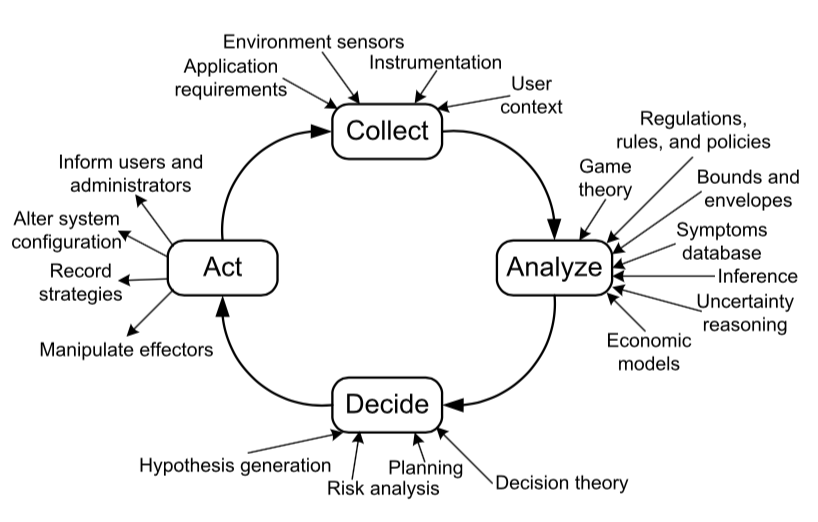
\includegraphics[width=0.8\textwidth]{imagens/generic-feedback-loop.png}
\caption{Ciclo de \textit{feedback} genérico \cite{dobson06}}
\label{generic-feedback-loop}
\end{figure}

Um exemplo da aplicação do clico de \textit{feedback} é discutido em \cite{brun09}. Os autores consideram que para manter os serviços Web em funcionamento durante um longo período de tempo requer a coleta de informações que reflitam o estado atual do sistema, analisando essas informações para diagnosticar problemas de desempenho ou para detectar falhas, decidindo como resolver o problema (por exemplo, via balanceamento dinâmico de carga ou corrigindo falhas), e agindo para efetuar as decisões tomadas.

Ao conceber um sistema adaptativo, algumas questões sobre essas atividades tornam-se importantes. Estas questões relativas aos laços de feedback devem ser explicitamente identificadas, registradas e resolvidas durante o desenvolvimento de um sistema adaptativo. A seguir serão apresentadas as questões levantas em \cite{brun09, lamprecht12}:

\begin{itemize}

\item O ciclo de \textit{feedback} começa com a coleta de dados relevantes de sensores disponíveis no ambiente e outras fontes que auxiliam na compreensão do estado atual do sistema. Algumas das questões que precisam ser respondidas aqui são: Qual é a taxa de amostragem necessária? Quão confiável é o dado do sensor? Existe um formato de evento comum entre os sensores? Os sensores fornecem informações suficientes para a identificação do sistema?;

\item Na sequência, o sistema analisa os dados coletados. Nesta etapa existem inúmeras abordagens para estruturar e raciocinar sobre os dados brutos (por exemplo, usando modelos, teorias e regras). Algumas das questões aplicáveis aqui são: Como o estado atual do sistema é inferido? Qual a quantidade/tempo de situações passadas podem ser necessárias no futuro? Quais dados precisam ser arquivados para validação, verificação e/ou conformidade? Quão fiel será o modelo ao mundo real e se um modelo adequado pode ser obtido a partir dos dados de sensores disponíveis? Quão estável será o modelo ao longo do tempo?;

\item Em seguida, uma decisão deve ser tomada para adaptar o sistema objetivando alcançar um estado desejável. Abordagens como análise de risco ajudam na escolha entre várias alternativas. Para esta atividade, as questões importantes são: Como o estado futuro do sistema é inferido? Como é alcançada uma decisão? Quais são as prioridades para a auto-adaptação em vários clicos de \textit{feedback} e em um único clico de \textit{feedback}?;

\item Finalmente, para implementar a decisão, o sistema deve agir por meio dos atuadores disponíveis. As questões importantes que surgem aqui são: Quando a adaptação deve e pode ser realizada com segurança? Como os ajustes de diferentes clicos de feedback interferem um ao outro? Os feedbacks centralizados ou descentralizados ajudam a atingir o objetivo global? Uma importante questão aplicável adicional é se o sistema de controle tem autoridade de comando suficiente sobre o processo, ou seja, se os atuadores disponíveis são suficientes para conduzir o sistema nas direções desejadas.

\end{itemize}

O modelo genérico de um clico de \textit{feedback} ilustrado na Figura \ref{generic-feedback-loop}, muitas vezes referido como o clico de controle autonômico, enfatiza as atividades que realizam feedback. Embora este modelo forneça um ponto de partida sobre os clicos de feedback, ele não detalha o fluxo de dados e o controle em torno do clico \cite{dobson06}. Ainda que esses clicos de feedback tenham tido muito sucesso em diferentes ramos de engenharia, como na teoria de controle, ainda não está claro se os princípios gerais desta disciplina podem ser aplicados diretamente em sistemas adaptativos. Diferentemente da teoria de controle, os cenários da IoT possuem uma estrutura não totalmente conhecida \cite{lamprecht12}.


Em uma tentativa de lidar com as complexidades dos sistemas modernos de computação a \textit{International Business Machines} (IBM) assumiu os desafios mencionados e sugeriu o modelo \textit{Monitor-Analyze-Plan-Execute plus Knowledge} (MAPE-K), conforme apresentado na Figura \ref{mape-k-model}. O MAPE-K utiliza as atividades Monitorar, Analizar, Planejar e Executar empregando um clico de controle em conjunto com o componente Conhecimento que fornece as informações necessárias para realizar a adaptação \cite{aman15}. O componente Monitor coleta os dados apropriados dos recursos gerenciados por meio dos sensores. Os dados são correlacionados, filtrados e/ou agregados e o sintoma descoberto é passado para o componente Analisar. Sintomas e outros dados também podem ser armazenados em uma base de conhecimento compartilhada. O analisador determina se uma mudança precisa ser feita com base no conhecimento compartilhado (potencialmente uma política) e nos sintomas. Caso pertinente, uma solicitação de mudança no ambiente é passada para o componente Planejar. O planejador gera os comandos ou fluxos de trabalho necessários na forma de um plano de alteração que é passado para o componente Executar. O executor aplica o plano de mudança no recurso de gerenciamento usando os atuadores. Caso necessário, a base de conhecimento pode ser atualizada, fornecendo dados do impacto da adaptação para serem aplicados como feedback para o próximo clico \cite{lamprecht12}.

\begin{figure}[ht]
\centering
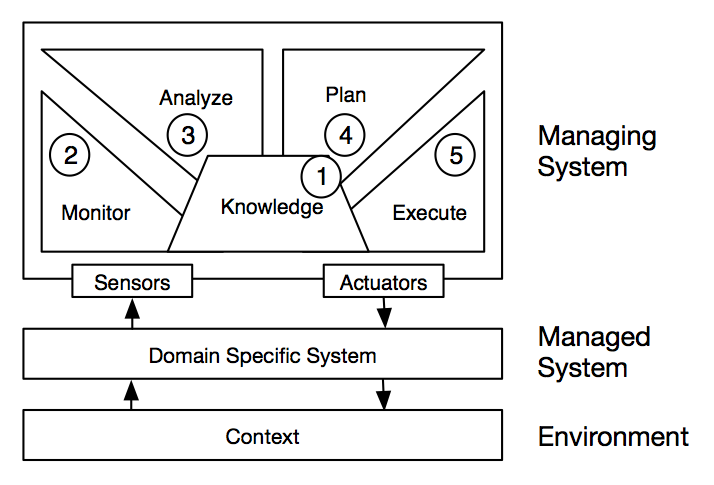
\includegraphics[width=0.8\textwidth]{imagens/mape-k-model.png}
\caption{MAPE-K - Modelo para sistema adaptativos \cite{iglesia15}}
\label{mape-k-model}
\end{figure}


De acordo com a IBM, um sistema autonômico deve ter os seguintes auto-atributos \cite{kephart03, iglesia15}: 

\begin{itemize}

\item Autoconfiguração (\textit{self-configuration}): o sistema deve se configurar automaticamente de acordo com as políticas de alto nível pré-definidas. Este atributo também contempla a facilidade de se adaptar às mudanças causadas por configurações automáticas. A integração, instalação e configuração de dispositivos e softwares devem ser feitos eficientemente. Caso a nova configuração não proporcione para a rede o desempenho esperado, há a possibilidade de restauração da mesma.

\item Auto-otimização (\textit{self-optimization}): consiste da habilidade do sistema controlar os recursos e os parâmetros de segurança para melhorar o desempenho e a eficiência, consequentemente aprimorando a qualidade dos serviços (QoS).

\item Autocura (\textit{self-healing}): é a capacidade do sistema detectar, diagnosticar e reparar falhas automaticamente sem que isto afete o funcionamento do sistema. A auto-cura é determinante na disponibilidade e confiabilidade do sistema.

\item Autoproteção (\textit{self-protection}): este atributo envolve dois aspectos: a defesa contra ataques e antecipação de ataques. A defesa deve ser realizada com o objetivo de protejer o sistema de ataques maliciosos ou falhas que não foram tratadas corretamente pela auto-cura. A antecipação de ataques é feita baseando-se em relatórios de sensores e, com essas informações, medidas devem ser adotadas para minimizar os problemas.

\end{itemize}

Em \cite{evesti13b}, os autores mencionam outros dois atributos, a autoconsciência (\textit{self-awareness}) e a ciência de contexto (\textit{context awareness}). A autoconsciência é a capacidade do sistema em conhecer seu próprio estado, seus componentes, capacidades, limites, recursos e comportamento. Já a ciência do contexto, consiste do conhecimento sobre o ambiente operacional ao qual o sistema está inserido. 


% gartner The Four Stages of an Adaptive Security Architecture???

%%%%%%%%%%%%%%%%%%%%%%%%%%%%%%%%%%%%%%%%%%%%%%%%%%%%%%%%%%%%%%%%%%%%%%%
\section{Ciência de Contexto na Segurança Adaptativa}

A ciência de contexto está presente nas pesquisas relacionadas a UbiComp, sendo um dos grandes desafios no desenvolvimento de aplicações nesta área.  Para entender o seu significado, primeiramente é necessário definir contexto, que de acordo com Dey (2001)\nocite{dey01} é qualquer informação que pode ser usada para caracterizar a situação de uma entidade (pessoa, local ou objeto) que é considerada relevante para a interação entre o usuário e a aplicação, incluindo o próprio usuário e a aplicação.

Contexto pode ser considerado também como uma descrição complexa de conhecimento compartilhado sobre circunstâncias físicas, sociais, históricas, entre outras, onde ações ou eventos ocorrem, percebendo assim a relação existente entre contexto e eventos. Contexto é o que contribui para a correta interpretação de uma ação ou evento, sem, no entanto, ser parte dessa ação/evento. Também pode ser considerado como sendo uma coleção de condições relevantes e influências que tornam uma situação única e compreensível \cite{brezillon99, li15}.

Existem seis questões básicas que podem ser realizadas para facilitar a compreensão do contexto, elas são conhecidas como 5W+1H \cite{vieira04}. No entanto, para determinadas aplicações algumas são mais importantes que outras. A seguir as seis questões são apresentadas:


\begin{itemize}

\item quem (\textit{who}): informação de presença e disponibilidade dos indivíduos no grupo, e de identificação dos participantes envolvidos num evento ou numa ação;

\item o quê (\textit{what}): informação sobre a ocorrência de um evento de interesse;

\item quando (\textit{when}): informação temporal sobre o evento, o momento em que o evento ocorreu;

\item onde (\textit{where}): informação espacial, de localização, o local onde o evento ocorreu;

\item por que (\textit{why}): informação subjetiva sobre as intenções e motivações que levaram à ocorrência do evento;

\item como (\textit{how}): informação sobre a maneira com que o evento ocorreu.

\end{itemize}

O contexto é relativo a um foco, onde foco pode ser uma tarefa ou um passo na resolução de um problema ou em uma tomada de decisão \cite{brezillon05}. Dessa forma, o foco determina onde está o contexto e o que pode ser considerado como importante, pois nem tudo que é contexto de uma situação é relevante para tal. 
 
As áreas da UbiComp e Inteligência Artificial foram as pioneiras nos estudos e utilização do conceito de contexto e, com isso, foram as que demonstraram o potencial da aplicação desse conceito nos sistemas computacionais. Ultimamente, a ciência de contexto vem sendo foco de um grande número de pesquisas dentro da UbiComp. Dessa forma, neste texto entende-se por ciência de contexto a capacidade de um sistema em usar o contexto para prover serviços e/ou informações relevantes para o usuário \cite{dey01}.

Ao se construir e executar aplicações ubíquas cientes de contexto há uma série de funcionalidades que devem ser providas, envolvendo desde a aquisição de informações contextuais, a partir do conjunto de fontes heterogêneas e distribuídas, até a representação dessas informações, seu processamento, armazenamento, e a realização de inferências para seu uso em tomadas de decisão \cite{bellavista12}. Tais tarefas se alinham ao clico de feedback empregado na formalização da segurança adaptativa.

Os sistemas cientes de contexto devem ser flexíveis, se adaptarem, e serem capazes de atuar automaticamente para ajudar o usuário na realização de suas atividades, o que está diretamente associado às necessidades das soluções para segurança da informação. Algumas motivações para usar a ciência de contexto são: 

\begin{itemize}

\item auxilia na compreensão da realidade;

\item facilita na adaptação de sistemas;

\item auxilia no processo de transformação dos dados em informação;

\item apoia a compreensão de eventos e de situações.

\end{itemize}

Em \cite{heimerl12},  é discutida a importância de contexto à segurança da informação. Inicialmente, ele defende a ideia de que informação sem contexto é simplesmente um dado, e não informação. Logo, dados são mais valiosos quando contextualizados.  Um cenário que exemplifica isto é apresentado em \cite{aman15}, onde é descrito um médico, atualmente em férias, usando seu smartphone. O mesmo recebe autorização por um Sistema de Controle de Acesso Baseado em Função, do inglês \textit{Role-Based Access Control} (RBAC), para acessar informações pessoais do paciente de um lugar incomum, em um fim de semana. Do ponto de vista do RBAC, esta atividade parece ser legítima, e o sistema deve conceder acesso. No entanto, se for analisado todo o contexto, isto é, o local incomum, o estado atual e a data de acesso, pode-se concluir que existe um risco envolvido se o acesso for concedido, ou seja, o smartphone pode ter sido comprometido. Portanto, para prover segurança adaptativa com eficiência deve-se avaliar a situação em um contexto holístico.

% Talvez colocar um outro exemplo
%\citealp{heimerl12} apresenta um exemplo, onde o autor considera uma solução de segurança relatando que o endereço IP 192.161.0.12 está passando por uma varredura de portas, no entanto, isto consiste simplesmente de uma parte dos dados. Ainda é  necessário descobrir o que esses dados significam ao analista de segurança, se seriam importantes ou somente ruído, logo, ele necessita identificar o contexto. Por exemplo, o alerta, que antes consistia apenas de um ``dado'' recebe um novo significado, o endereço IP 192.161.0.12 hipoteticamente pode ser o sistema que mantém o banco de dados dos cartões de créditos dos alunos de uma universidade, ou pode ser  um site interno que não tem valor real para a instituição.

%Embora, o contexto do alerta tenha sido aprimorado, ainda é possível supor que o servidor que está sendo atacado é chamado de ``sentinela'', e é um Windows Server 2008 R2 SP1, rodando Oracle 11g Enterprise, que está localizado em Pelotas, Rio Grande do Sul, Brasil, na linha 3 do \textit{data center}, prateleira A12, e que detém todos os registros de pacientes clínicos, abrangendo assim as normas \textit{Health Insurance Portability and Accountability Act} (HIPAA) e \textit{Health Information Technology for Economic and Clinical Health} (HITECH). Percebe-se que a contextualização dos dados é importante no processo de aquisição de informação, e que possui uma grande diferença na maneira como a informação é gerenciada e protegida, tornando-se relevante para segurança da informação.

No que tange a segurança adaptativa, caso os contextos relevantes para a identificação das situações a serem avaliadas não sejam adequadamente levadas em consideração, pode haver uma influência adversa no ambiente impactando nos serviços oferecidos. Observa-se que a segurança adaptativa, é fortemente dependente do ambiente monitorado e da visão holística sobre o mesmo. Em outras termos, a contextualização deve ocorrer em diferentes níveis arquiteturas (desde a coleta do evento, passando pela normalização, análise de risco e assim por diante). A ciência de contexto é especialmente crítica nos cenários da IoT, em particular na adaptação, pois esta consiste de uma comunicação máquina para máquina, a priori sem a inteligência (envolvimento direto) dos humanos. Caso sejam levados em consideração contextos irrelevantes, incorretos ou insuficientes, a adaptação pode não ser eficiente \cite{aman15}.



\section{Considerações sobre o Capítulo}

Inicialmente neste capítulo foi apresentada a definição de IoT, sendo destacado que a segurança adaptativa é considerado um desfio importante e atual. Posteriormente a segurança adaptativa foi discutida, sendo exposto que o uso de um clico de \textit{feedback} se faz necessário para apoiar a implantação deste conceito. Também foi descrito que a ciência de contexto é um atributo fundamental para a adaptação. Com isto, na seção seguinte foi analisada a ciência de contexto descrevendo como ela pode ser aplicada neste âmbito.


\chapter{Embasamento Teórico}
Para fornecer um embasamento teórico ao leitor sobre a Ciência de Situação que será discutida no capitulo \ref{cap:Estado_da_Arte} será abordado nas seções seguintes deste capitula as definições assumidas neste documento para evento, processamento de evento, processamento de fluxo de eventos e processamento de eventos complexos respectivamente.

\section{Definição de Evento}
A definição de evento considerada neste documento é definida como a ocorrência de uma determinada ação dentro de um ambiente, que geralmente envolve uma tentativa de mudança de estado do sistema. A qual inclui normalmente a noção de tempo, localidade e detalhes pertencentes ao evento ou a anomalia que desencadeou determinado evento que visam ajudar a compreender as causas ou efeitos desencadeadores do evento \cite{fitzgerald2010common}.
Um evento também pode ser separado em campos que descrevem suas propriedades, como por exemplo um evento em uma rede IoT pode incluir quatro atributos: eventID, eventName, eventTime e recordTime. EventID e eventName são normalmente definidos como registros básicos e são armazenados no data center, eventTime e recordTime expressam o conceito de tempo no evento descrevendo sua hora de ocorrência e de captura respectivamente \cite{minbo2013information}. 

Tais eventos podem ser aplicados em diversos sistemas para se atingir determinados fins, como por exemplo o uso em ferramentas de monitoramento onde estes eventos são utilizados para representar mudanças em situações \cite{etzion2011event}. Estes sistemas monitorados podem ser representados por conjuntos de sensores, onde por exemplo, em aplicações na agricultura de precisão são usados para o monitoramento da umidade e acidez do solo, de forma que tais valores emitidos por estes sensores podem ser vistos como mudanças de estado do ambiente, como uma mudança brusca na acidez do solo ou em sua umidade, as quais podem ser representadas como uma mudança de situação de interesse \cite{garcia2011wireless}.

\section{Definição de Processamento de Evento}
O processamento de eventos (\textit{Event processing} - EP) pode ser visto como um paradigma onde fluxos de eventos são analisados continuamente com o objetivo de extrair informações uteis de alto nível destes dados analisados. Existem diversas áreas que possuem características com potencial de serem exploradas pelo processamento de eventos, dentre estas podemos citar os setores da saúde com o monitoramento do status da saúde dos paciente onde os diversos eventos precisam ser processados e analisados \cite{weiner2008health}; o setor da agricultura de precisão o qual emprega diversos sensores para o monitoramento de plantas, gerando grandes fluxos de eventos que necessitam ser processados \cite{garcia2011wireless} e o setor de energia fazendo uso de eventos para o monitoramento do consumo excessivo de energia visando atingir uma eficiência energética melhor \cite{vijayaraghavan2010automated}. 

Apesar do processamento de eventos ser aplicado para resolver problemas em áreas totalmente distintas, existem alguns requisitos exigidos por estes que são normalmente semelhantes, tais como a necessidade de processar em tempo de execução grandes volumes de dados. Um setor em constante  crescimento que tem gerado grandes interesses no processamento de eventos é a Internet das Coisas(\textit{Internet of Things} - IOT) onde processamento de eventos tem se aplicado visando solucionar problemas de tomadas de decisão a partir da analise de grandes volumes de dados gerados por estas redes, diversas ferramentas foram desenvolvidas para o processamento de eventos, visando auxiliar na analise desse grande volume de dados, dentre estas podemos citar o Apache Storm\footnote{\url{https://storm.apache.org/}}, Apache Spark\footnote{\url{https://spark.apache.org/}} e Apache Flink\footnote{\url{https://flink.apache.org/}}.

O processamento de eventos é uma grande área de pesquisa, onde podemos dividir esta em outras duas principais subáreas: Processamento de fluxo de eventos(\textit{event stream processing} - ESP), a qual tem a capacidade de executar operações continuas sob fluxos de dados como filtros, agregações, classificações e junções; Processamento de eventos complexos (\textit{complex event processing} - CEP) usa padrões pré definidos, sobre sequencias de eventos simples, para fazer a detecção de eventos compostos (\cite{dayarathna2018recent}), a figura \ref{fig:ConjuntoProcessamento} ilustra esta associação entre estas classes de eventos.


\begin{figure}[ht]
	\centering
	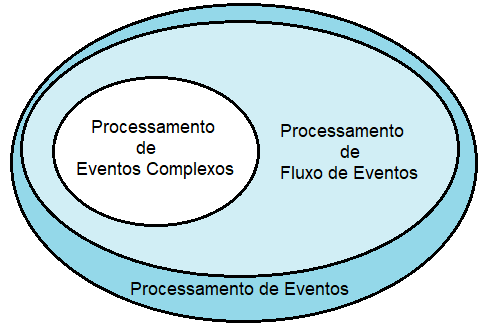
\includegraphics[width=.6\textwidth]{imagens/ConjuntoProcessamento.png}
	\caption{Conjunto de associação de processamento.}
	\label{fig:ConjuntoProcessamento}
\end{figure}


\section{Definição de Processamento de Fluxo de Eventos}

Para termos uma melhor e simples compreensão do significado de processamento de fluxo de eventos (\textit{Event Stream Processing} - ESP) podemos separar esta classe em outras três subclasses menores:
\begin{enumerate}
\item  \textbf{Evento -} podemos definir evento neste contexto como qualquer ação que aconteça com um tempo claramente definido, onde o mesmo pode ser mensurado.  

\item  \textbf{Fluxo -} é definido como um sequencia constante e continuo de eventos disparados por dispositivos, onde esta corrente de eventos são claramente ordenados pelo tempo.

\item  \textbf{Processamento} - é basicamente a ação final de executar a analise sobre o conjunto de informações capturadas.
\end{enumerate}
Desta forma com a combinação destes três sub-termos podemos dizer que o processamento de fluxo de eventos nada mais é que processo de analisar em tempo de execução fluxo de eventos disparados por dispositivos assim que estes são criados \cite{dayarathna2018recent}. 

O processamento de fluxo de dados trada da identificação de padrões ou relacionamentos significativos entre os fluxos de dados analisados afim de detectar determinados padrões como a correlação de eventos, causalidade ou tempo.
Características presentes em sistemas com aplicabilidade de processamento de fluxo de eventos são a necessidade de analisar grandes fluxos de dados correlacionando estas informações, aplicando filtros em tempo de execução e dando uma resposta de forma imediata, \cite{appel2013event}.


\section{Definição de Processamento de Eventos Complexos}
O processamento de eventos complexos (\textit{Complex Event Processing} - CEP) é uma tecnologia recente normalmente aplicada para o processamento em tempo real de fluxos de informações em sistemas baseados em eventos, sistemas que empregam esta tecnologia normalmente apresentam as seguintes características: o processamento de dados em tempo de execução; um grande fluxo de eventos que precisam ser analisados; a necessidade de combinar para assim executar a analise destes eventos a qual não pode ser executada de forma trivial; e eventos que são produzidos de fontes distintas (fontes de dados heterogêneas). Uma área com grande aplicabilidade para o processamento de eventos complexos que tem se destacado nos últimos anos é a Internet das Coisas que apresentam grandes fluxos de dados de fontes heterogêneas e que normalmente necessitam ser analisados em tempo de execução \cite{jun2014design}. 

Assim para definirmos o conceito de processamento de eventos complexos tomado no desenvolvimento deste documento, executaremos uma separação  deste termo mais complexo em outros dois sub-conceitos menores que o compõe com o objetivo de facilitar a sua compreensão, Processamento e eventos complexos onde podemos definir processamento como o ato final de analisar as informações já coletadas pelo sistema e eventos complexos como um forma evento nova mais abstrata de alto nível inferida a partir de eventos simples. Mais especificamente podemos definir um evento complexo como sendo a combinação de dois ou mais eventos simples com o objetivo de criar um novo evento de mais alto nível, por exemplo \cite{dayarathna2018recent}, em um data center onde sensores monitoram o uso do disco rígido do sistema e o uso de rede, os eventos de alto uso do disco repentinamente disparam, após a analise destes eventos o sistema pode "decidir" disparar um novo evento "possível ataque Hacker" onde a partir deste novo evento os administradores podem decidir tomar alguma decisão  baseada neste novo evento como por exemplo desligar da rede do data center \cite{wu2006high}. 

Assim quando combinamos estes dois sub-conceitos citados temos que o processamento de eventos complexos é o ato de analisar em tempo de execução grandes fluxos de eventos complexos isto é, eventos inferidos a partir de conjuntos de eventos simples, com o objetivo de extrair algum conceito de mais alto nível.  



%%%%%%%%%%%%%%%%%%%%%%%%%%%%%%%%%%%%%%%%%%%%%%%%%%%%%%%%%%%%%%%%%%%%%%% 
\chapter{Estado da Arte} 
\label{cap:Estado_da_Arte}

Neste capítulo é apresentado o estado da arte das pesquisas que tem como tema processamento de eventos e internet das coisas. Na seção seguinte é apresentado o protocolo seguido para a execução do mapeamento sistemático assim como todos os passos executados que levaram a escolha dos trabalhos de interesse. Por fim será apresentado uma discussão sobre as soluções abordadas nos trabalhos de interesse selecionados.    

\section{Mapeamento Sistemático da Literatura}

O mapeamento sistemático abordado neste capítulo é baseada na metodologia proposta por Petersen et al. (2008), onde seguindo a série de passos proposto, torna o estudo realizado, possível de ser replicado por outros pesquisadores \cite{petersen08}. A partir desta metodologia, pode ser citado cinco etapas das quais serão seguidas por este mapeamento:

\begin{enumerate}
	\item Definição das questões de pesquisa;
	\item Execução da pesquisa para identificação de estudos primários realizados;
	\item Triagem, inicial empregando critérios de inclusão e exclusão considerando o resumo dos artigos;
	\item Triagem final, considerando as seções de introdução, concepção do projeto e conclusão;
	\item Extração dos dados e mapeamento.
	

\end{enumerate}  

Para a consulta dos trabalhos relacionados primeiramente foi definido um conjunto de palavras como candidatas a palavras chave para a \textit{string} de busca, dentre estas podemos citar: \textit{internet of things}, \textit{distributed} e \textit{complex event processing}. A Partir da definição destas como palavras chave, foi possível elaborar a \textit{string} de busca usada para executar as consultas sobre as bases da: ACM Digital Library, IEEE Explore, ScienceDirect, Springer, Web of Science e Scopus; e assim obter-se os trabalhos relacionados com o tema de pesquisa, as strings de consulta podem ser vistas na figura \ref{tab:stringBusca} incluindo em qual respectiva base estas foram executadas.



\begin{figure}[ht]
	\centering
	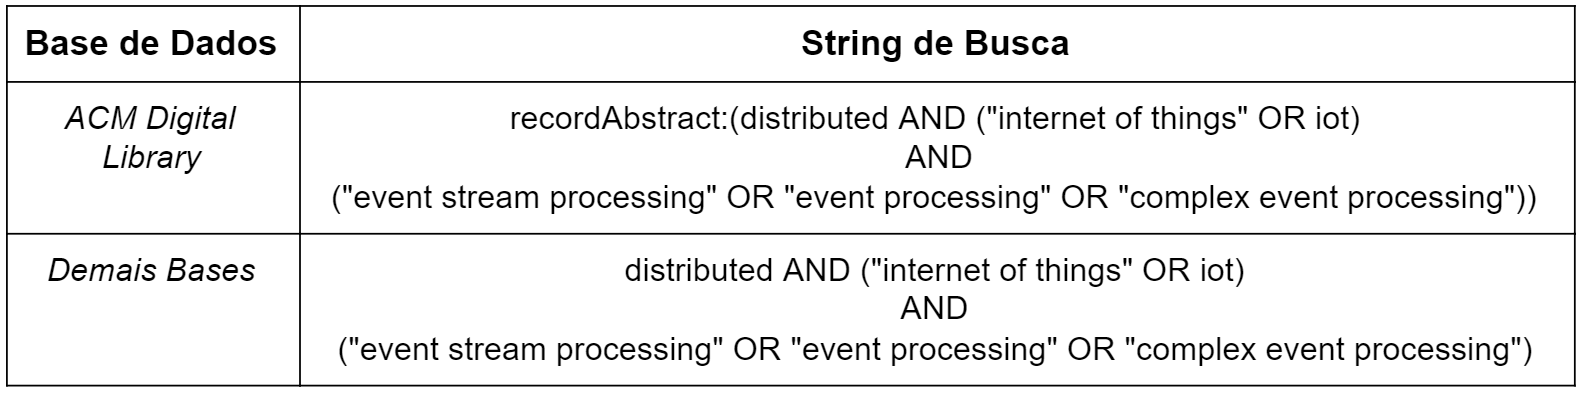
\includegraphics[width=1\textwidth]{imagens/tabela_string_busca.png}
	\caption{Strings de buscas usadas.}
	\label{tab:stringBusca}
\end{figure}

Após a execução desta consulta preliminar, que entende-se como a etapa de levantamento dos estudos primários relevantes, foram identificado 647 trabalhos de interesse onde este valor  compreende-se da soma dos resultados obtidos em todas as bases de consulta.

Todas as buscas foram realizadas sobre os metadados dos artigos(titulo, resumo e palavras chave), porem, como a base de dados Springer não oferecia suporte a este tipo de consulta, este problema foi contornado da seguinte forma: primeiramente foi feita a exportação do resultado preliminar da busca na base para o formato CSV(o único suportado) resultando em 472 artigos. Após isto fez-se uso da ferramenta CSV2Bib\footnote{\url{https://github.com/jacksonpradolima/csv2bib}} para converter o arquivo CSV para .bib com o intuito de importar o resultado, para a ferramenta Zotero\footnote{\url{https://www.zotero.org/}}, oque permitiu a execução da String de busca sobre os metadados dos 472 artigos encontrados preliminarmente, resultando em 6 documentos de interesse. A figura  \ref{fig:GrafBarraPubAno} apresenta um gráfico de barras contendo o número de artigos encontrados pela \textit{string} de busca em cada uma das bases, já a figura \ref{fig:GrafPizPubAno} apresenta o percentual de publicações que cada uma das bases contribuiu para o montante final.

\begin{figure}[ht]
	\centering
	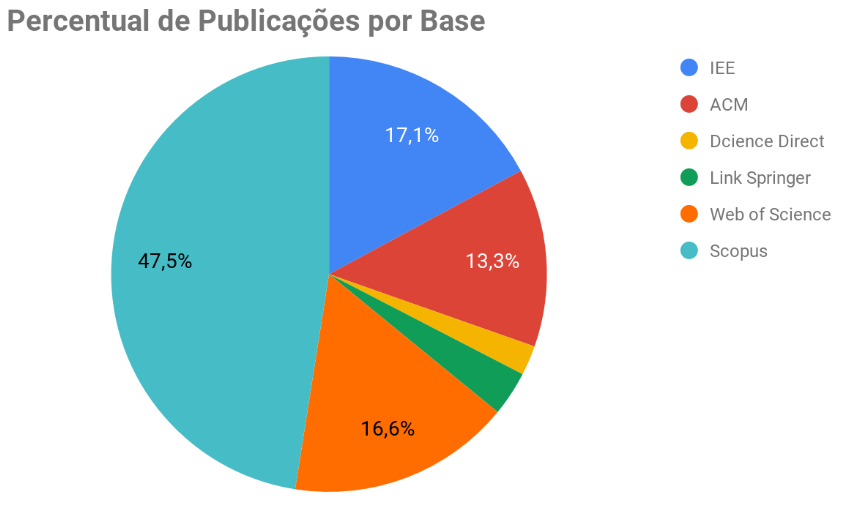
\includegraphics[width=.9\textwidth]{imagens/GrafPizPubAno.png}
	\caption{Percentual de publicações encontradas por base.}
	\label{fig:GrafPizPubAno}
\end{figure}

\begin{figure}[ht]
	\centering
	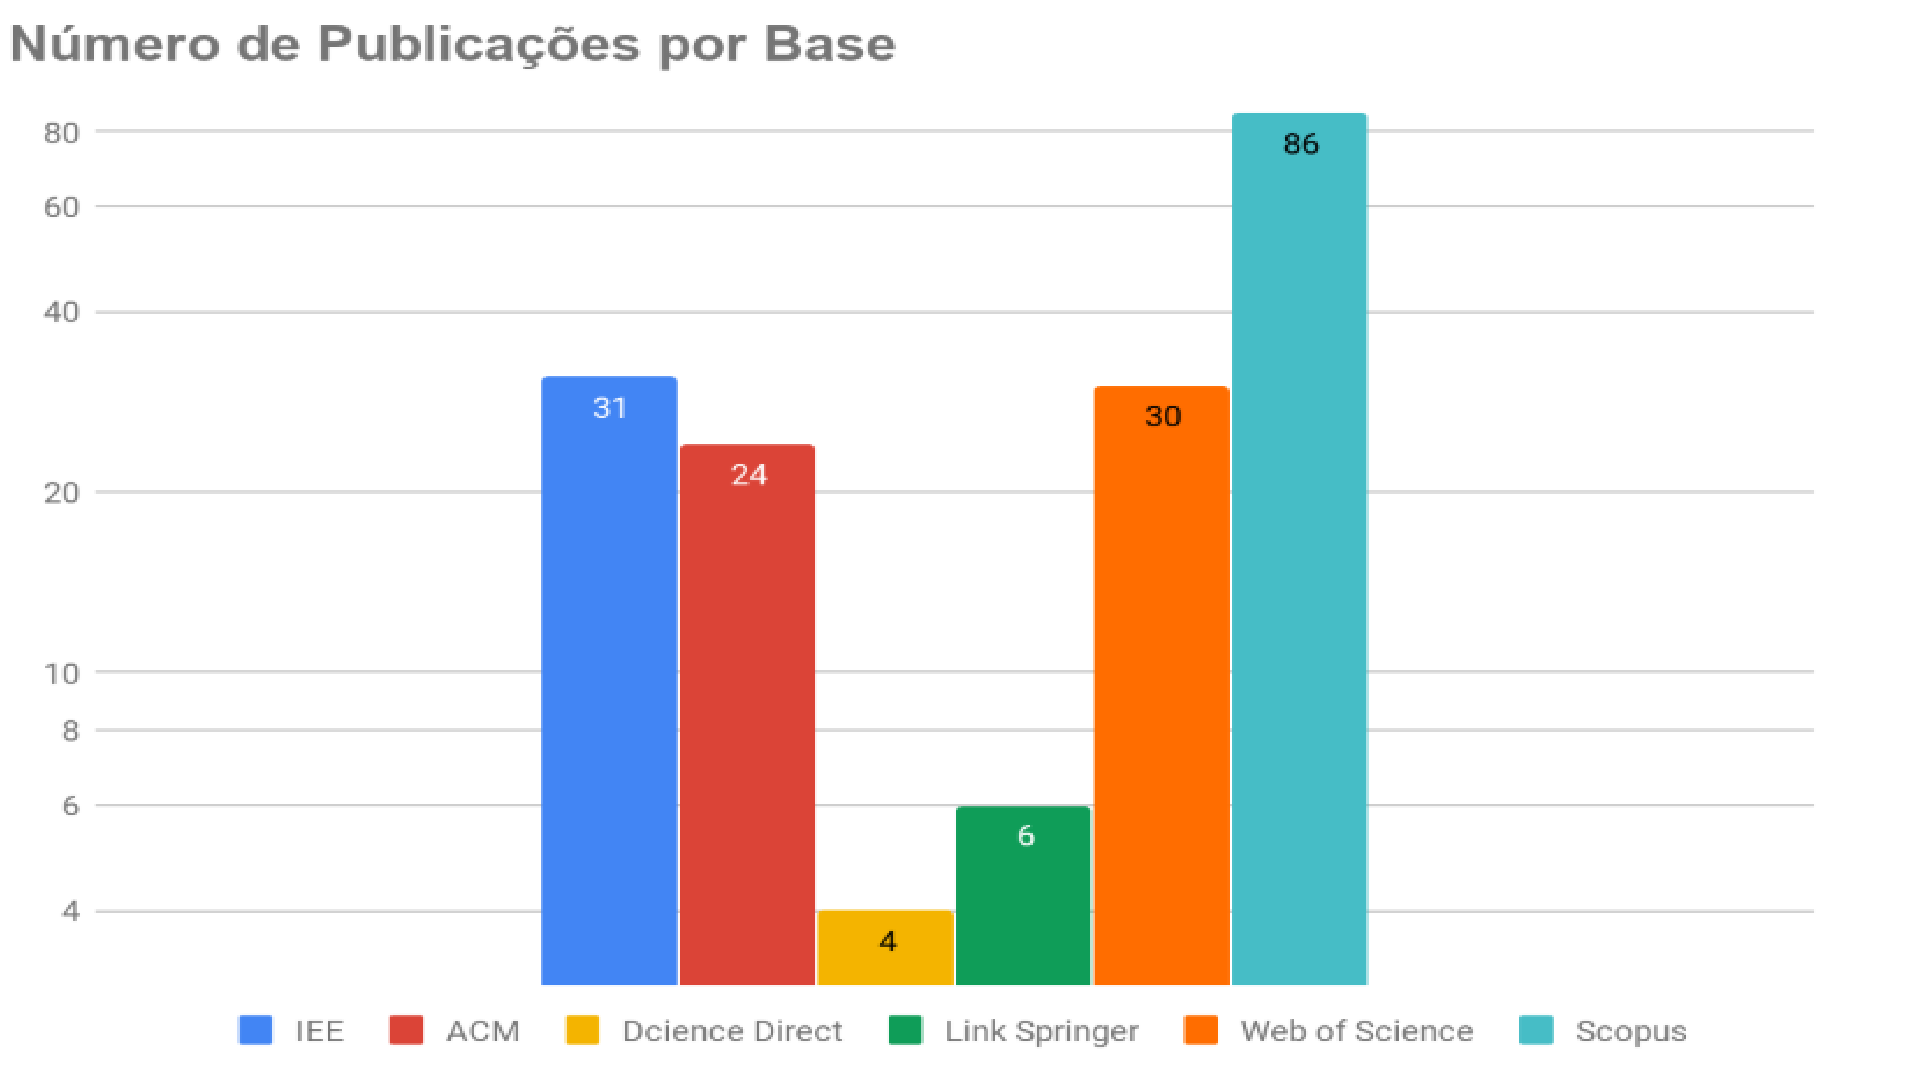
\includegraphics[width=.9\textwidth]{imagens/GrafBarraPubAno.png}
	\caption{Número de publicações encontradas por base.}
	\label{fig:GrafBarraPubAno}
\end{figure}


O gráfico \ref{fig:grafPublicaAno} apresenta o número de publicações de interesse encontradas e cada uma das bases. O eixo X apresenta o ano do qual os artigos foram publicados e o eixo Y apresenta o número total de publicações em relação ao ano. Para a representação do gráfico foram removidas todas as publicações duplicadas. Podem-se perceber pela figura \ref{fig:grafPublicaAno} que a partir do ano de 2015 há um considerável aumento no número de publicações, e ainda um grande pico no ano de 2017, demonstrando assim pontos de interesse neste período de publicações.

\begin{figure}[ht]
	\centering
	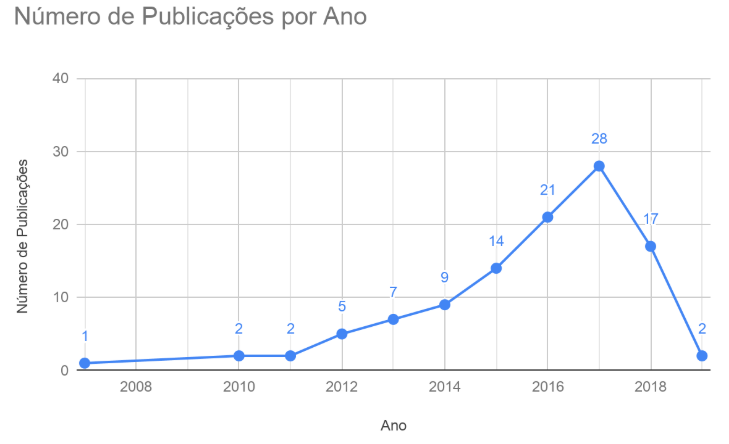
\includegraphics[width=.9\textwidth]{imagens/grafPublicaAno.png}
	\caption{Quantidade de publicações de interesse por ano.}
	\label{fig:grafPublicaAno}
\end{figure}

\subsection{Critérios de Inclusão e Exclusão}
Após a seleção inicial realizada sobre as bases de dados, executou-se a triagem inicial sobre o resumo dos artigos, aplicando os seguintes critérios de inclusão e exclusão conforme a ordem apresentada abaixo: 
\begin{itemize}
	\item (E) Foi publicado antes de 2015;
	\item (E) Não é um artigo \textit{full paper};
	\item (E) Não esta em Inglês ou Português;
	\item (E) Indisponibilidade de acesso ao artigo completo;
	\item (E) Artigos que não apresentam avaliação da proposta;
	\item (I) Explora conceitos de segurança;
	\item (I) Explora conceitos de Computação Ubíqua;
	\item (E) O artigo não possui nenhum dos critérios de inclusão.
\end{itemize}
	
Para auxiliar na aplicação dos critérios de inclusão e exclusão foi feita a importação dos resultados preliminares das buscas na ferramenta Start\footnote{\url{http://lapes.dc.ufscar.br/tools/start_tool}},
para isso usou-se os arquivos .bib exportados pelas ferramentas das bases de busca, com exceção apenas da Spriger, onde usou-se o arquivo .bib exportado pelo Zootero, que foi gerado apos a execução da consulta sobre os metadados, aplicada sobre o resultado preliminar da base.

Os critérios de exclusão foram aplicados seguindo a seguinte ordem e etapas:

\begin{itemize}
	\item  \textbf{Remoção de Trabalhos Duplicados - } Muitos dos trabalhos retornados pela \textit{string} de busca estavam indexados em ambas as bases de consulta, tornando necessário a execução de uma etapa de remoção dos mesmos, resultando em 74 trabalhos duplicados removidos.
	
	\item  \textbf{Filtro por Data - } O intervalo de interesse para a aplicação do filtro foi adotado com base no número de publicações por ano. Após o levantamento dos trabalhos de interesse, identificou-se o ano de 2015 como sendo o ano em que o número de publicações aumenta considerável mente, continuando a ascender até o pico máximo no ano de 2017, como pode ser visto na figura \ref{fig:grafPublicaAno}. Assim optou-se por eliminar todas as publicações que fossem anteriores ao ano de 2015 eliminando desta forma 26 artigos.	
	
	\item  \textbf{Artigos Full Paper - } Com o intuito de remover artigos que apresentassem apenas resumos superficiais sobre os trabalhos, ou que não tivesse apelo científico, optou-se por remover artigos que não sejam Full Paper (livro ou capítulo de livro, introdução de anais, entre outros), sendo removidos 9 trabalhos.
	
	\item  \textbf{Filtro por Idioma - } Como as pesquisas foram realizadas sobre varias bases de dados onde muitas destas indexam trabalhos em vários idiomas, optou-se por usar um filtro por idioma para remover qualquer trabalho que não esteja em Português ou Inglês(idiomas de total domínio do autor) removendo desta forma 1 artigo.
	
	\item  \textbf{Indisponibilidade do Artigo completo - } Dado que alguns dos estudos de interesse selecionados apresentaram apenas seus resumos e introdução disponíveis não oferecendo a opção de obter-se o trabalho completo, optou-se por remover estes do pesquisa, sendo excluído 3 trabalhos.
	
	\item  \textbf{Avaliação da Proposta - } Foram removidos todos os artigos que não executaram algum tipo de teste ou estudo de caso das soluções propostas por seus trabalhos, excluindo assim 17 artigos.
	
	\item  \textbf{Sem Nenhum Critério de Inclusão - } Todos trabalhos que não  se enquadraram em nenhum dos critério de inclusão foram removidos, excluindo desta forma 28 trabalhos da pesquisa.	

\end{itemize}


Após execução da triagem inicial dos trabalhos, aplicando os critérios de inclusão e exclusão sobre o resumo dos artigos, selecionou-se 24 documentos de interesse, o fluxo da aplicação dos critérios de exclusão pode ser visto na figura \ref{fig:grafFluxoTriagemInicial} assim como o número total de trabalhos removidos por cada um dos critérios de aplicação. 

A execução da 4º etapa do mapeamento, que consiste da triagem final dos trabalhos de interesse, selecionou dez dos 24 artigos para analise completa de seu conteúdo e da extração das informações destes. O critério considerado para a seleção dos dez trabalhos foi se estes exploravam conceitos de segurança da informação ou ainda se estes apresentavam o uso de conceitos de Computação Ubíqua. 


\begin{landscape}
\begin{figure}[ht]
	\centering
	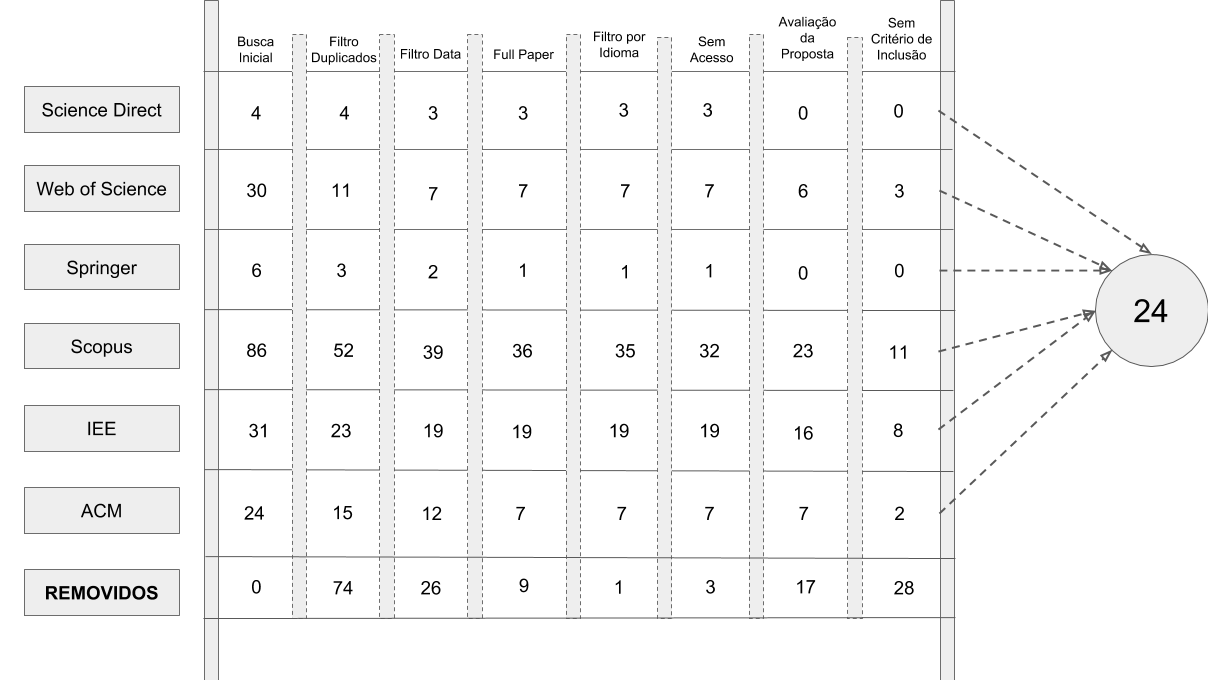
\includegraphics[width=1.7\textwidth]{imagens/FluxoTriagemInicial.png}
	\caption{Fluxo de triagem dos artigos.}
	\label{fig:grafFluxoTriagemInicial}
\end{figure}
\end{landscape}


\section{Trabalhos Relacionados}
Com a execução do mapeamento sistemático da literatura
foram selecionados dez trabalhos de interesse, os quais serão apresentados nas subseções a seguir, onde serão abordados os seguintes tópicos de interesse: motivação e justificativa do trabalho, solução apresentada, avaliação e Resultados da Proposta.


%%%%%%%%%%%%%%%%%%%%%%%%%%%%%%%%%%%%%%%%%%%%%%%%%%%%%%%%%%%%%%%%
\subsection{Towards a Generalized Approach for Deep Neural Network based Event Processing for the Internet of Multimedia Things}


\begin{itemize}
	\item \textbf{Motivação e Justificativa do Trabalho:} O uso de dispositivos IoT multimídia tem aumentado consideravelmente (uso de câmeras para monitorar o trafego de uma cidade por exemplo). Desta forma os tipos dos eventos criados na IoT estão também mudando, onde estes eventos multimédia geram dados não estruturados, gerando uma procura crescente na utilização eficiente do processamento de fluxos de eventos multimídia. No entanto, os mecanismos de processamento de eventos atuais têm suporte limitado ou inexistente para tipos de evento não estruturados.
	
	\item \textbf{Solução Apresentada:} É proposto um sistema genérico para manipular eventos da Internet das Coisas Multimídia (IoMT) como um tipo de evento nativo em ferramentas de processamento de eventos com alta eficiência. O sistema proposto estende as linguagens de processamento de eventos com a introdução de operadores para análise multimídia de eventos não estruturados (eventos multimídia) e aproveita um combinador de eventos baseado em rede neural convolucional profunda para processamento de eventos de imagem, para extrair recursos.
	
	\item \textbf{Avaliação e Resultados da Proposta:} O sistema desenvolvido foi otimizado usando uma abordagem de seleção de classificador baseada em restrições de assinatura. Os resultados obtidos mostram que a ferramenta atinge uma taxa de transferência média de 110 quadros/segundo com uma precisão aproximada de 66,34\% em eventos do mundo real de várias aplicações de cidades inteligentes. Foi apresentado ainda um teste de desempenho com o aumento do número de classes por classificador, onde os resultados obtidos mostram uma taxa de transferência estável para um classificador de uma classe, porem com o aumento do número de classes a taxa de transferência cai continuamente.  
	
\end{itemize}


\subsection{A Web-based Approach using Reactive Programming for Complex Event Processing in Internet of Things Applications}

\begin{itemize}
	\item \textbf{Motivação e Justificativa do Trabalho:} Nos últimos anos a Internet das coisas (IoT) tem crescido substancialmente, aumentando progressivamente o número de dispositivos conectados a rede, estima-se que em poucos anos cada um dos objetos de uso comum irá conter sensores para coletar e/ou fornecer algum tipo informação ou serviço para seus usuários, se conectando na Internet e gerando cada vez mais uma enorme quantidade de dados para serem trafegados pela rede. Esse crescente aumento no número de dispositivos e consequentemente a grande expansão no volume de dados, gera a necessidade que seja desenvolvida uma abordagem simples para que se possa lidar com esta nova grande avalanche de dados.
	
	\item \textbf{Solução Apresentada:}  Foi proposto a combinação de duas abordagens distintas para a solucionar o problema citado da nova grande avalanche de dados gerados pelas redes IoT: a CEP(\textit{Complex Event Processing}) e WoT (\textit{Web of Things}) com o uso de Ferramentas gráficas que exploram programação de fluxo (Mashups) o que irá permitir o uso de operadores CEP em eventos de alto niveis visualmente criados na plataforma WoT.
	Para o desenvolvimento dos operadores CEP utilizou-se Programação Reativa, os quais foram fornecidos como uma extensão da plataforma WoT Node-RED\footnote{\url{https://nodered.org/}}, onde foram implementado três dos programas Coral8 amplamente referenciados para sistemas CEP, gerando a primeira extensão do CEP para a plataforma Node-RED, esta sendo uma ferramenta de programação construída em cima do Node.js, como protocolo de comunicação da troca de mensagens, os autores optaram por usar o MQTT\footnote{\url{https://mqtt.org/}}(\textit{Message Queuing Telemetry Transport}) . 	
	
	\item \textbf{Avaliação e Resultados da Proposta:} Para a avaliação da proposta do trabalho, um cenário de caso de uso é apresentado onde para este proposito usou-se o simulador node-red-node-pi-sense-hatsimulator, desenvolvido pela equipe Node-RED que tem como objetivo reproduzir uma placa real Raspberry PI a qual incorpora alguns sensores e atuadores como LEDs, temperatura, pressão barométrica e sensores de umidade, entre outros, os quais foram usados para a simulação dos CEP da proposta. Com o desenvolvimento deste trabalho os autores citaram duas como as principais contribuições da pesquisa: (1) uma abordagem visual para construir consultas CEP para aplicativos de Internet e (2) o uso de Programação Reativa para detectar e acionar o CEP.
	
\end{itemize}


\subsection{Semantic IoT Middleware-enabled Mobile Complex Event Processing for Integrated Pest Management}

\begin{itemize}
	\item \textbf{Motivação e Justificativa do Trabalho:} Existem diversos desafios na agricultura moderna que são tipicamente encontrados no domínio dos Sistemas Ciber-Físicos (CPSs), dentre estes pode ser citado: conhecimento e deficiência de infraestrutura, informações incompletas, fontes limitadas de informação, perturbações externas (clima), autoridade de controle limitada (fertilizantes não podem fazer uma planta crescer arbitrariamente rápido). O gerenciamento agrícola moderno depende  de muitas metodologias diferentes de sensoriamento para fornecer informações precisas sobre a cultura, o clima e as condições ambientais. Graças a miniaturização, da grande evolução e da difusão de sensores e recursos computacionais de baixo custo, tornou-se possível o desenvolvimento de dispositivos que produzem dados e que interagem entre sí, produzindo assim uma rede de "coisas", gerando dados, processos e serviços interconectados. Desta forma os CPSs estão transformando a indústria agrícola.
	
	\item \textbf{Solução Apresentada:} O trabalho propõe uma infraestrutura inteligente projetada para processar fontes de dados heterogêneas, como dados de sensores, dados meteorológicos e conhecimento agrícola coletado em uma ontologia, possibilitando uma comunicação mais suave e homogênea entre os dispositivos de uma infraestrutura dinâmica, configurável e extensível. A solução desenvolvida é baseada em processamento de eventos complexos (CEP) com o uso da ferramenta Esper, onde um modulo é executado parcialmente em dispositivos móveis através da introdução do DeviceHive, um \textit{middleware} da Internet das Coisas (IoT), ainda fez-se uso de uma linguagem de programação com suporte a mecanismos de reflexão, os quais servem como uma interface entre os componentes da IoT e o conhecimento ontológico. Para o sistema de comunicação entre o servidor e os dispositivos moveis é usado um \textit{middleware} de publicação/assinatura composto por um DSB (\textit{Distributed Service Bus}), um serviço do \textit{Google Cloud Messaging} e um serviço da Web de assinatura. Segundo os autores a solução visa tornar-se um instrumento utilizado para conscientizar sobre o uso dos tratamentos agrícolas, onde o agricultor pode (i) ter acesso a todas as informações relacionadas ao domínio de interesse no momento necessário, (ii) criar um plano de defesa personalizado, (iii) receber alertas de mudanças nas condições climáticas e (iv) receber notificações e recomendações sobre seus planos de tratamento.

	
	\item \textbf{Avaliação e Resultados da Proposta:} Para a validação da proposta desenvolvida foi apresentado uma instanciação de um cenário real, projetando também uma Ontologia OWL(\textit{Ontology Web Language}) que codifica o conhecimento sobre aspectos relacionados à prática de Manejo Integrado de Pragas. Também os autores executaram um primeiro conjunto de experimentos para validar a abordagem de fornecer a ferramenta para uma empresa e testar componentes individuais. Por fim os autores citaram como principais contribuições do trabalho: (i) a possibilidade de usar o motor CEP em tempo de execução do sistema, o que permite o monitoramento orientado a eventos e notificações de atualização, e (ii) sistema de modelagem com ontologias compreensíveis homem-máquina, que garante uma reconfiguração mais fácil a ferramenta. 
	
\end{itemize}

\subsection{Predictive Analytics for Complex IoT Data Streams}

\begin{itemize}
	\item \textbf{Motivação e Justificativa do Trabalho:} Os CEP são capazes de fornecer soluções escaláveis e distribuídas para lidar com fluxos de dados complexos em tempo real, no entanto, os CEPs  não possuem a capacidade de realizar predições assim como muitas das técnicas de aprendizado de máquina e análise estatística de dados. A grande parte dos aplicativos CEP disponíveis  na literatura destina-se apenas a fornecer soluções reativas ao correlacionar fluxos de dados usando regras predefinidas, não explorando dados históricos devido a sua memória limitada. Existem diversos casos em que a predição de um evento futuro é muito mais útil que apenas a detecção do mesmo, por exemplo, seria muito mais útil a previsão de um congestionamento em uma auto estrada do que sua detecção, já que a predição deste com certa antecedência, torna-se possível informar aos administradores de trafego, para que estes possam tomar as medidas preventivas de modo a evitar o congestionamento. Podemos citar ainda diversos outros casos onde a predição de eventos futuros podem trazer diversos ganhos como a previsão de desastres naturais e doenças epidêmicas. 
	
     \item \textbf{Solução Apresentada:} Neste trabalho foi proposto uma arquitetura pró-ativa capaz de explorar dados históricos usando técnicas de aprendizado de máquina em conjunto com processamento de eventos complexos, de forma a combinar o poder do processamento de dados em tempo real do CEP com a capacidade de predição de eventos das técnicas de ML. Foi apresentado um algoritmo de predição adaptativo chamado de AMWR (\textit{Adaptive Moving Window Regression}) para dados dinâmicos de IoT, capaz de realizar predições precisas quase que em tempo real, e ainda sendo capaz de trabalhar em conjunto com o CEP. Para a execução da proposta foram utilizados: Node-RED para fornecer o Front-End da arquitetura, o Apache Kafka\footnote{\url{https://kafka.apache.org/}} como Broker de mensagens e por ultimo, a implementação foi elaborada em Python com o módulo de aprendizagem de máquina scikit-learn.  
     
     
     
	 \item \textbf{Avaliação e Resultados da Proposta:}
	 Para avaliação da proposta foi elaborado um caso de uso do mundo real onde dados de trafego de sistemas de transportes inteligentes foram usados para os testes, onde o algoritmo de predição foi capaz de atingir uma precisão de 96\%, demonstrando assim a sua viabilidade de uso, já que com predições corretas sobre o trafego, como as que foram apresentadas nos testes, permitem que os administradores do sistema gerenciem o tráfego de uma maneira melhor, tomando decisões para evitar situações indesejadas, como congestionamentos por exemplo.	 
	 Os autores do artigo citam como principais contribuições do trabalho:
	 a implementação de uma arquitetura genérica baseada em componentes de código aberto para combinar ML com CEP, a fim de prever eventos complexos para aplicativos proativos de IoT;
	 o desenvolvimento de um algoritmo de predição adaptativo para fluxos de dados dinâmicos de IoT que foi implementado em um caso de uso real do ITS atingindo uma precisão de até 96\%. Também foi proposto um novo método para encontrar tamanho ótimo para janela de treinamento, explorando componentes espectrais de dados de séries temporais;
	 A modelagem do erro introduzido pelo algoritmo de previsão usando uma distribuição paramétrica e a derivação em expressões para o erro global do sistema, à medida que o erro se propaga através do CEP.
\end{itemize}


\subsection{DRESS: A Rule Engine on Spark for Event Stream Processing}

\begin{itemize}
	\item \textbf{Motivação e Justificativa do Trabalho:} Nos últimos anos o número de dispositivo conectados a rede vem aumentando, com esse crescimento, a quantidade de fluxos de dados aumenta simultaneamente, gerando a necessidade de sistemas capazes de reagir automaticamente a determinados eventos desencadeados por fluxos de dados. Tais sistemas se baseiam em um conjunto de regras pre definidas, onde através da análise dos fluxos de informações, executam determinadas ações que satisfação a alguma das regras deste conjunto. Nas últimas três décadas, sistemas como estes têm sido amplamente empregados em empresas, governos e organizações. Porém o aumento crescente no tamanho dos fluxos de dados, como o grande número de fluxos produzidos por eventos de dispositivos da Internet of Things (IoT), faz com que os atuais sistemas baseados em regras enfrentem sérios desafios em termos de velocidade, escalabilidade e tolerância a falhas.
	
	\item \textbf{Solução Apresentada:} O artigo apresenta a proposta de adaptar sistemas baseados em regras para trabalhar em conjunto com o Spark Streaming visando melhorar seu desempenho. Foi apresentado uma Transformação do algoritmo Rete, que está por trás de muitos dos \textit{Rule based systems} (RBSs) atuais, esta transformação faz com que o algorítimo funcione como um mecanismo de regras no ambiente do Spark. Também foi introduzido juntamente com um novo sistema de mensagens baseado em Kafka o DRESS (\textit{Distributed Rule Engine no Spark Streaming}) onde foi demonstrado uma forma automatizada de transformar regras escritas no estilo do Apache Drools para serem executadas no DRESS, tornando fácil para os atuais usuários do Drools mover seus sistemas para o DRESS sem esforço, este método de transformação de regras é baseada em técnicas MDA e na biblioteca de usuários SiTra.
	
	\item \textbf{Avaliação e Resultados da Proposta:} O sistema proposto foi avaliado com a ajuda de um estudo de caso, onde foi simulado um sistema bancário para a execução dos testes. Os autores usaram o DRESS para transformar as regras CEP definidas para o ambiente de estudo, em código Scala e assim executá-lo no Spark Streaming. Um gerador de dados foi criado com o intuito de produzir informação aleatoriamente para a simulação do ambiente bancário, incluindo fluxos de caixa, contas e períodos contábeis com um parâmetro de escala. Durante os testes o DRESS demonstrou uma melhora significativa de desempenho e escalabilidade em comparação ao Drools, demonstrando ser capaz de lidar com grandes volumes de dados, em contra partida, o Drools não demonstrou esta mesma capacidade. Além  da alta capacidade de processamento, o DRESS se demonstrou mais flexível em termos de gerenciamento de memória, mesmo nos testes executados em uma única máquina, este pode processar um conjuntos de dados maiores que o Drools e em menos tempo. Assim os autores destacam que com os dados coletados pelo estudo de caso, se pode demonstrar que o DRESS tem potencial para resolver muitos dos problemas de processamento de grande fluxo de dados presentes nos RBSs.
	
\end{itemize}

\subsection{TrustCEP: Adopting a Trust-Based Approach for Distributed Complex Event Processing}


\begin{itemize}
	\item \textbf{Motivação e Justificativa do Trabalho:} O avanço da Internet das Coisas(IoT), com o uso de sensores modernos e dispositivos moveis capazes de capturar grandes quantidades de informações, estimulou o desenvolvimento de aplicativos aptos a trabalhar com essa nova grande avalanche de informações. Uma técnica eficaz que surgiu com o objetivo de extrair informações contextuais de alto nível deste grande fluxo de dados foi o CEP(\textit{Complex Event Processing}), facilitando a analise de dados em tempo real provenientes de fontes heterogêneas e distribuídas. Considerando que o contexto dos usuários pode ser de informações sensíveis, a preservação da privacidade destes dados é critica, tendo em vista que o processamento do contexto do usuário pode ocorrer em vários dispositivos (possivelmente maliciosos), especialmente em cenários colaborativos. Os trabalhos atuais sobre processamento de eventos complexos geralmente negligenciam o nível de privacidade dos dados do contexto de seus usuários onde estes são processados e diferentes dispositivos, muitas vezes com níveis de segurança desconhecidos. 
	
	
	\item \textbf{Solução Apresentada:} Para solucionar o problema de controle de privacidade, os autores propõem uma abordagem baseada em confiança, onde usam esta métrica de confiança definida para o posicionamento e a execução de operadores CEP em ambientes distribuídos, atribuindo o processamento de dados sensíveis para dispositivos que tenham um nível de confiança mais alto. Para a definição deste valor, a ferramenta pode usar o histórico de interação entre os dispositivos, ou ainda usar uma funcionalidade de recomendações de confiança, a qual faz uma verificação de similaridade baseada em cosseno, evitando assim ataques de collusion e on-off. Como as fontes de informações em um ambiente IoT são decentralizadas o modelo do sistema construído escolhido pelos autores foi entorno de uma rede device to device(D2D).
	
	
	\item \textbf{Avaliação e Resultados da Proposta:} Para a validação da proposta, um sistema CEP foi desenvolvido de forma distribuída baseado em SmartPhones, o qual possibilita aos usuários se comunicarem com uso de Bluetooth e processar gráficos de maneira distribuída. Esta ferramenta foi chamada de TrustCEP a qual foi usada para avaliar a abordagem. Para medir as relações de confiança, foi gerado um histórico de interações entre usuários em canais síncronos e assíncronos, os quais representam aspectos comportamentais da confiança dos usuários. Como métricas de comparação foram usados o consumo médio de energia e a troca de dados na rede, onde os autores observaram que com a implementação da proposta os smartPhones usados para os testes apresentaram um leve aumento de 2-6\% no consumo de energia, se comparado a abordagens quem não levam em consideração a privacidade dos dados, em contra partida o modelo proposto se mostra robusto contra ataques collusion e on-off.
	Os autores citam como principais contribuições de seu trabalho: o desenvolvimento de um modelo de gestão de confiança (descentralizada) para adaptar a disseminação de eventos e a colocação de operadores para o CEP distribuído; Foi introduzido um modelo de gestão de confiança baseado nas relações do usuário e no histórico de interação de comunicação; Foi apresentado um esquema de recomendação de confiança robusto usando a medida de similaridade de cosseno.
	
	
\end{itemize}

\subsection{Anaysis of Controller Based IEEE 802.11 System with Similarity Measure Clustering}

\begin{itemize}
	\item \textbf{Motivação e Justificativa do Trabalho:} A eficiência de um sistema WiFi que contenha dezenas de estações em uma área física pequena, em suma, é dada pela capacidade do sistema de alocar de forma ótima canais de rede para estas estações de forma a evitar conflitos de frequências ns rede ao máximo. Com a evolução dos dispositivos moveis, com alta capacidade de trafego de dados, sua grade popularização e seu uso acentuado em locais densamente povoados como por exemplo o uso de smartphones em grandes edifícios, se faz necessário o desenvolvimento ferramentas inteligentes capazes de oferecer bons níveis de QoS aos usuários. Para a configuração dos canais em um modo de operação normal uma rede WiFi usa o algoritmo de gerenciamento de recursos de rádio (RRM) onde este é executado periodicamente. Sendo definido vários valores de configurações nos pontos de acesso para iniciar tarefas de gerenciamento adicionais no controlador entre os períodos, as quais podem ser enxergadas como eventos complexos. Devido à complexidade, esses parâmetros para os valores do algoritmo RRM são normalmente fornecidos como valores padrões. Existindo uma falta significativa de experiências práticas sobre os operadores de serviço WiFi em busca dos valores ideais.
	
	
	
	\item \textbf{Solução Apresentada:} Como proposta do trabalho os autores levantam as seguintes questões de: Qual é o nível real de desempenho de um determinado sistema WiFi configurado com o controlador? Quão sensato é este algoritmo RRM para futuros ataques de inundação nos canais de rádio em um AP ou terminal móvel? Com o intuito de responder a estas questões levantadas, os autores propõe a execução de uma análise profunda deste sistema onde estes usam uma  abordagem de análise estatística baseada em mecanismos de agrupamento de comportamento e detecção de mudanças, fazendo a analise das informações coletadas para assim chegar a uma conclusão final. Alem disso os autores também propõem um novo método de clustering baseado em medidas de similaridade e aplicado nas redes Wifi IEEE 802.11.
		
	
	\item \textbf{Avaliação e Resultados da Proposta:} Para a validação da proposta do trabalho, foram executadas as medições do sistema WiFi na rede de informática da Universidade de Debrecen, os autores também ressaltam que as medições das duas tecnologias WiFi relativas as bandas de 2,4 GHz e 5 GHz foram analisadas separadamente. Após a execução dos testes sobre as redes wifi da universidade, os autores concluem que o método de clustering baseado em comportamento proposto, é capaz de avaliar o desempenho do algoritmo de gerenciamento de recursos de rádio do controlador WiFi de forma eficiente, sendo capaz de informar os valores reais de desempenho que os AP produzem com a configuração do algoritmo padrão e gerar os valores ótimos mais adequados para aquela rede.
	
	
\end{itemize}


\subsection{Parallel big data processing system for security monitoring in Internet of Things networks*}

\begin{itemize}
	\item \textbf{Motivação e Justificativa do Trabalho:} Atualmente as redes de Internet das Coisas (IoT) tem se popularizado em diversas áreas. Assim como a sua popularização, a preocupação com a segurança dessas redes tem aumentado, levando ao interesse de desenvolvimento de sistemas de segurança sofisticados para a proteção destas redes, os quais são necessários ja que o uso de sistemas de proteção tradicionais são de difícil ou impossível aplicação devido às peculiaridades para a construção e operação de redes IoT. Pode-se citar como fatores complicantes na implementação de sistemas de segurança nas redes IoT como: a necessidade de analisar grandes quantidades de dados em tempo real com o menor custo computacional possível, grande número de fontes de dados heterogêneas, computação limitada e recursos de energia limitado. Outro fator que destaca a importância de sistemas de segurança para redes IoT é a grande variedade de ataques cibernéticos existentes e a gravidade de suas consequências. Sistemas de informações de segurança e gerenciamento de eventos (SIEM) tem a capacidade de monitorar a segurança de redes por meio da coleta de dados sobre: eventos de interesse de dispositivos remotos, sensores de informação e seu processamento preliminar. Porém redes IoT possuem um grande número de tipos de fontes de dados, o que pode tornar extremamente complexo o monitoramento da segurança de rede devido a alta intensidade de fluxos de eventos, levando a necessidade do desenvolvimento de sistemas de segurança com capacidade de processamento de Big Data.
	
	\item \textbf{Solução Apresentada:} Levando em consideração as limitações citadas para o desenvolvimento de sistemas de segurança para redes IoT, o trabalho propõe uma nova arquitetura de segurança para redes IoT baseada em um sistema de processamento paralelo distribuído de Big Data. A ferramenta de processamento de dados paralelo desenvolvido tem as seguintes características: devido ao uso da tecnologia CEP (Processamento de Eventos Complexos), o sistema implementa funções básicas de pré-processamento em tempo real, as quais são: normalização de dados, filtragem de dados, agregação de dados e correlação de dados; os resultados do processamento preliminar dos dados são fornecidos pela representação visual do sistema; a ferramenta é configurada para operar sob condições de limitações computacionais, inerentes aos elementos de rede da IoT. Para o desenvolvimento do sistema de processamento paralelo de dados de segurança, foi usado como base a ferramenta de código aberto Hadoop\footnote{\url{https://hadoop.apache.org/}} em conjunto com o ambiente de processamento de dados distribuído Apache Spark. A arquitetura do sistema também inclui componentes responsáveis pela coleta, armazenamento, agregação, normalização, análise e visualização de dados onde: a Agregação dos dados, normalização, análise e visualização são realizadas "on-the-fly"; Os dados são armazenados em um sistema de arquivos distribuídos do HDFS(\textit{Hadoop Distributed File System}), proporcionando um aumenta da confiabilidade do armazenamento e da velocidade com que as solicitações de dados são processadas.
	

	\item \textbf{Avaliação e Resultados da Proposta:} Para avaliação da proposta do artigo os fluxos de dados usados para os testes foram obtidos combinando fluxos de eventos de segurança em um fragmento da rede IoT com fluxos representados em um banco de dados externo de tráfego em uma rede real de computadores. A avaliação aplicada mostrou que, mesmo em um ambiente IoT com recursos computacionais limitados quando o sistema executa com o Hadoop, a ferramenta desenvolvida apresenta um desempenho razoavelmente alto, excedendo significativamente as implementações conhecidas, porem quando este é executado no Apache Spark a ferramenta mostrou um aumento de desempenho de cerca de dez vezes, caso o ambiente apresentar uma quantidade de memoria RAM suficiente. Como principais contribuições do trabalho os autores citam: a execução de um comparativo de desempenho das plataformas Hadoop e Spark implementadas em uma sistema de segurança de redes aplicado a IoT; o desenvolvimento de uma arquitetura destinada ao processamento paralelo e ao monitoramento de redes IoT. 
	
	
	
	
\end{itemize}


\subsection{An integrated information lifecycle management framework for exploiting social network data to identify dynamic large crowd concentration events in smart cities applications}

\begin{itemize}
	\item \textbf{Motivação e Justificativa do Trabalho:} Com o advento de novas tecnologias, como a Internet das Coisas e o processamento em nuvem, há uma grande diversidade de fontes de dados e serviços distintos disponíveis. O que nos leva a questão de como pode-se identificar maneiras inteligentes, abstratas e adaptativas de correlacionar e combinar os vários níveis de informações disponíveis gerados por estas novas tecnologias. Com o cenário tecnológico atual podemos destacar que o maior desafio dentre as questões levantadas é o de combinar diferentes fontes de dados heterogêneas de maneira inteligente, integrando e raciocinando sobre este fluxo de informação para inferir a consciência situacional, transformando desta forma o conjunto de dados brutos e sem significado para o nível de conhecimento e sabedoria dando um sentido semântico para estas informações. Para lidar com estes desafios, há necessidade do desenvolvimento de uma estrutura de \textit{big data} de analise concisa capaz de analisar e lidar com o grande fluxo de dados gerado por ambientes IoT.	
	
	\item \textbf{Solução Apresentada:} O objetivo do trabalho é o desenvolvimento de uma plataforma \textit{Smart Transportation} capaz de identificar eventos de interesse do usuário em uma determinada área (como grandes eventos públicos com alta concentração de pessoas que possam afetar a jornada do usuário), a fim de enriquecer as informações no nível de aplicação com a identificação de eventos relacionados que podem permitir ações mais sofisticadas em nome deste usuário, a identificação é baseada na observação dos picos de atividade do Twitter em comparação com os dados históricos em um tempo dinâmico e local de interesse. O sistema proposto inclui os seguintes aspectos: integração entre dados de cidades inteligentes, proveniente de um sistema específico de monitorização de passageiros da cidade de Madrid e dados de redes sociais provenientes do Twitter, para alertar passageiros com necessidades especiais e seus cuidadores sobre Grandes Concentrações de Multidões ao longo de sua jornada; Ingestão de dados integrados em soluções escaláveis baseadas em nuvem (OpenStack Swift) e integradas com ferramentas de análise de dados (Apache Spark) para trabalhar diretamente nos conjuntos de dados adquiridos e atuando com o processamento de eventos complexos (CEP), a fim de monitorar e emitir alertas de dados de fluxo. Ainda a solução deverá ser capaz de se adaptar a dados heterogêneos ajustando ao modelo Apache AVRO; Conexão de todos esses sistemas com uma lógica baseada em aplicações, obtida através de uma camada de \textit{middleware} baseada no NodeRED, a fim de orquestrar as ações necessárias no fluxo de dados previsto e fornecer as adaptações necessárias em termos de protocolos e formatos de dados.	
	
	\item \textbf{Avaliação e Resultados da Proposta:} Para validação do sistema proposto, a ferramenta foi aplicada em um experimento de dois meses na cidade de Madri, em torno de dois locais de eventos públicos, atuando na identificação de eventos de grandes concentrações de pessoas como eventos esportivos e analisando várias abordagens com relação à definição de limiares necessários como: estrutura integrada e automatizada, incluindo serviços da plataforma \textit{Smart City} e Twitter. Com este estudo de caso os autores obtiveram 49 erros de 2042 casos de avaliação, onde destes erros existiram apenas 4 falsos negativos. Porém como o sistema é flexível, este pode ser ajustado para especificações mais rígidas objetivando diminuir falsos positivos ou falsos negativos dependendo da preferencia do usuário.
	Ainda os autores citam como principais contribuições do trabalho: o desenvolvimento de um \textit{middleware} para adaptação e sincronização necessária do sistema, a execução de um experimento de 2 meses na cidade de Madri, o desenvolvimento de um sistema de identificação detalhado da concentração  de multidões por meio da localização dada com o uso de dados de redes sociais (Twiter), a identificação de limiares ideais para ignorar intervalos de tempo baseando-se em limites gerais de funções de distribuição cumulativas (CDF).
\end{itemize}


\subsection{CEML: Mixing and moving complex event processing and machine learning to the edge of the network for IoT}

\begin{itemize}
	\item \textbf{Motivação e Justificativa do Trabalho:} A internet das coisas (IoT) é um campo em constante crescimento. As previsões mostram que em 2020 mais de 50 bilhões de dispositivos conectados, levando a uma avalanche de informações gerada constantemente por estes dispositivos, onde muito deste grande aumento na quantidade de informação gerada se dá graças ao desenvolvimento de hardwares de baixa potência e protocolos de rede mais eficientes. Atualmente já existem muitos setores da industria que acumulam um grande volume de informação(por exemplo serviços investimento, mídia, bancos) as quais poderiam ser usadas por aplicações de exploração para gerar algum tipo de beneficio para estas entidades. Sistemas de análise em nuvem altamente escalonáveis estão sendo usados para lidar com esta explosão de dados gerada pelas redes IoT. Porém devido a natureza onipresente desses dados, á novos requisitos técnicos e não técnicos que são de difícil resolução com uma implantação em nuvem. Precisamos de um novo conjunto de tecnologias para resolver estes problemas, como mineração de dados distribuída e mineração de dados ubíqua desenvolvidas e otimizadas especialmente para a aplicação IoT.
	
	\item \textbf{Solução Apresentada:} Os autores propõem um novo \textit{framework} denominado \textit{Complex Event Machine Learning}(CEML) o qual apresenta um conjunto de ferramenta para aprendizado de maquina, distribuído automaticamente em ferramentas de avaliação contínuas automáticas em tempo real e gerenciamento automático de regras para a implementação de regras, onde estes recursos são desenvolvidos para uma implantação de borda de rede ou em nuvem. A ferramenta desenvolvida pelos autores apresenta os seguintes aspectos: Capaz de lidar com fluxos contínuos de dados através das instruções de fluxo do mecanismo CEP; não há requisitos de memória o qual é permitido pelo uso de mecanismos CEP em janelas de fluxo permitindo o uso inteligente da memória conforme necessário; o sistema é capaz de transferir resultados de mineração por uma rede sem fio com largura de banda limitada tratado pelo protocolo MQTT com o uso do Mosquitto Broker\footnote{\url{https://mosquitto.org/}}; a ferramenta é capaz de modelar as mudanças dos dados ao longo da execução já que o CEML é um modelo de aprendizagem de maquina os modelos usados por este se ajustam conforme aprendem; Um ambiente de mineração iterativo fornecido por uma API REST; Integração entre sistemas de gerenciamento de fluxo de dados e abordagens de mineração através da API REST. A ferramenta proposta foi desenvolvida a partir do Data-Fusion Manager, um micro-serviço LinkSmart® baseado em Java para \textit{Smart Cities}, o desenvolvimento do sistema de coleta de dados foi feito usando o broker Mosquitto e o cliente Paho Java, por fim para a implementação dos algorítimos de inteligencia artificial foi usado a API do Weka. 
	
	\item \textbf{Avaliação e Resultados da Proposta:} Para a avaliação do sistema proposto, foi executada a monitoração do desempenho da ferramento em uma implantação incorporada em um problema de classificação de tempo real aplicada para melhorar o sistema de detecção de presença na Universidade Federal de Pernambuco (UFPE) o qual apresentou um desempenho satisfatório durante os testes. Os autores validaram a proposta também em um ambiente de mais fácil reprodução, assim estes usaram um conjunto de dados da íris onde cada um destes dados foi enviado pela rede, assim como se fosse capturado por algum sensor,  onde estas informações são recebidas por um Broker implantado em uma Raspberry PI2 e processadas no mesmo pela ferramenta proposta de aprendizado, as medidas foram enviadas a uma média de 19,17 por segundo, sendo usado o algorítimo NaiveBayesUpdateable que foi capaz de apresentar bons resultados durante as medições.
	
	
	
\end{itemize}

\section{Discussão dos Trabalhos Relacionados}

Conforme destacado na introdução deste trabalho, de acordo com a literatura (em especial alguns ``\textit{surveys}''), inclusive com os trabalhos identificados no estado da arte, os seguintes aspectos foram identificados como problemas relacionados as pesquisas em arquiteturas/modelos de segurança adaptativa:

\begin{enumerate}
\item  se concentram em apenas um serviço/objetivo de segurança, como a autenticação \cite{aman14}, \cite{elkhodary07};
\item as abordagens existentes não definem todo o ciclo de adaptação MAPE \cite{yuan12}.
\item fornecem uma arquitetura genérica sem detalhar os métodos usados em cada componente  \cite{aman14}, \cite{yuan12};
\item a falta de detalhes nas arquiteturas genéricas dificulta a reutilização e extensibilidade das abordagens propostas \cite{yuan12};
\end{enumerate}

No que diz respeito ao primeiro e segundo problemas elencados, o mapeamento sistemático buscou filtrar esta questão, sendo selecionados apenas artigos onde as arquiteturas/modelos concebidos podem ser aplicados em diferentes objetivos de segurança e que contemplam o ciclo MAPE por inteiro. Já quanto ao terceiro e quarto tópicos levantados, é possível observar que o primeiro trabalho apresentado neste capítulo \cite{habtamu12} - o qual é concebido por uma das referências na área (Abie Habtamu) - possui tal limitação, a qual é tratada apenas em alguns dos demais trabalhos.

Tendo estas observações em vista, a tabela \ref{comparacao-estado-da-arte} busca apresentar algumas das características consideradas para comparação entre os trabalhados identificados como estado da arte em segurança adaptativa para IoT. O sinal de hífen (``-'') na tabela representa a falta de informações ou limitação por parte do trabalho quanto a referida característica. A seguir é apresentada uma breve descrição das características selecionadas:

\begin{itemize}
\item coleta: uma dos desafios na IoT diz respeito a coleta de eventos de dispositivos com recursos limitados, logo, esta característica busca identificar se são destacados no trabalho os detalhes para coleta dos eventos;
\item normalização: uma vez que o foco é na IoT, a heterogeneidade e a consequente diversidade no formato dos eventos produzidos deve ser tratada, sendo assim, este tópico identifica se a proposta detalha a estratégia utilizada para normalização;
\item correlação: estratégia utilizada para correlação dos diferentes contextos identificados para identificação de situações de interesse;
\item armazenamento: determina a tecnologia de armazenamento do conhecimento empregada, sendo relevante por fatores de expressividade, escalabilidade e usabilidade;
\item implementação: visa caracterizar o nível de detalhamento do protótipo desenvolvido para validação do trabalho, podendo ser 
``Não'', ``Parcial'' e ``Sim'';
\item extensibilidade: representa a possibilidade de extensão da arquitetura/modelo proposto;
\item reusabilidade: busca evidenciar se o trabalho descreve detalhes suficientes que permitem o reuso da proposta, sendo passível de replicação dos testes realizados;
\item maturidade: descreve o nível de maturidade da abordagem em função da validação desenvolvida e da comunidade em torno das tecnologias empregadas;
\item cenário: caracteriza a área de estudo do cenário de avaliação;
\item escalabilidade: procura identificar limitações ou competências quanto a escalabilidade da proposta uma vez que na IoT o volume de dados tratados em função da quantidade de dispositivos adquirindo contextos é um desafio a ser considerado.
\end{itemize}

\begin{table}[ht]
\centering
\caption{Tabela comparativa entre os trabalhos identificados como estado da arte em segurança adaptativa}
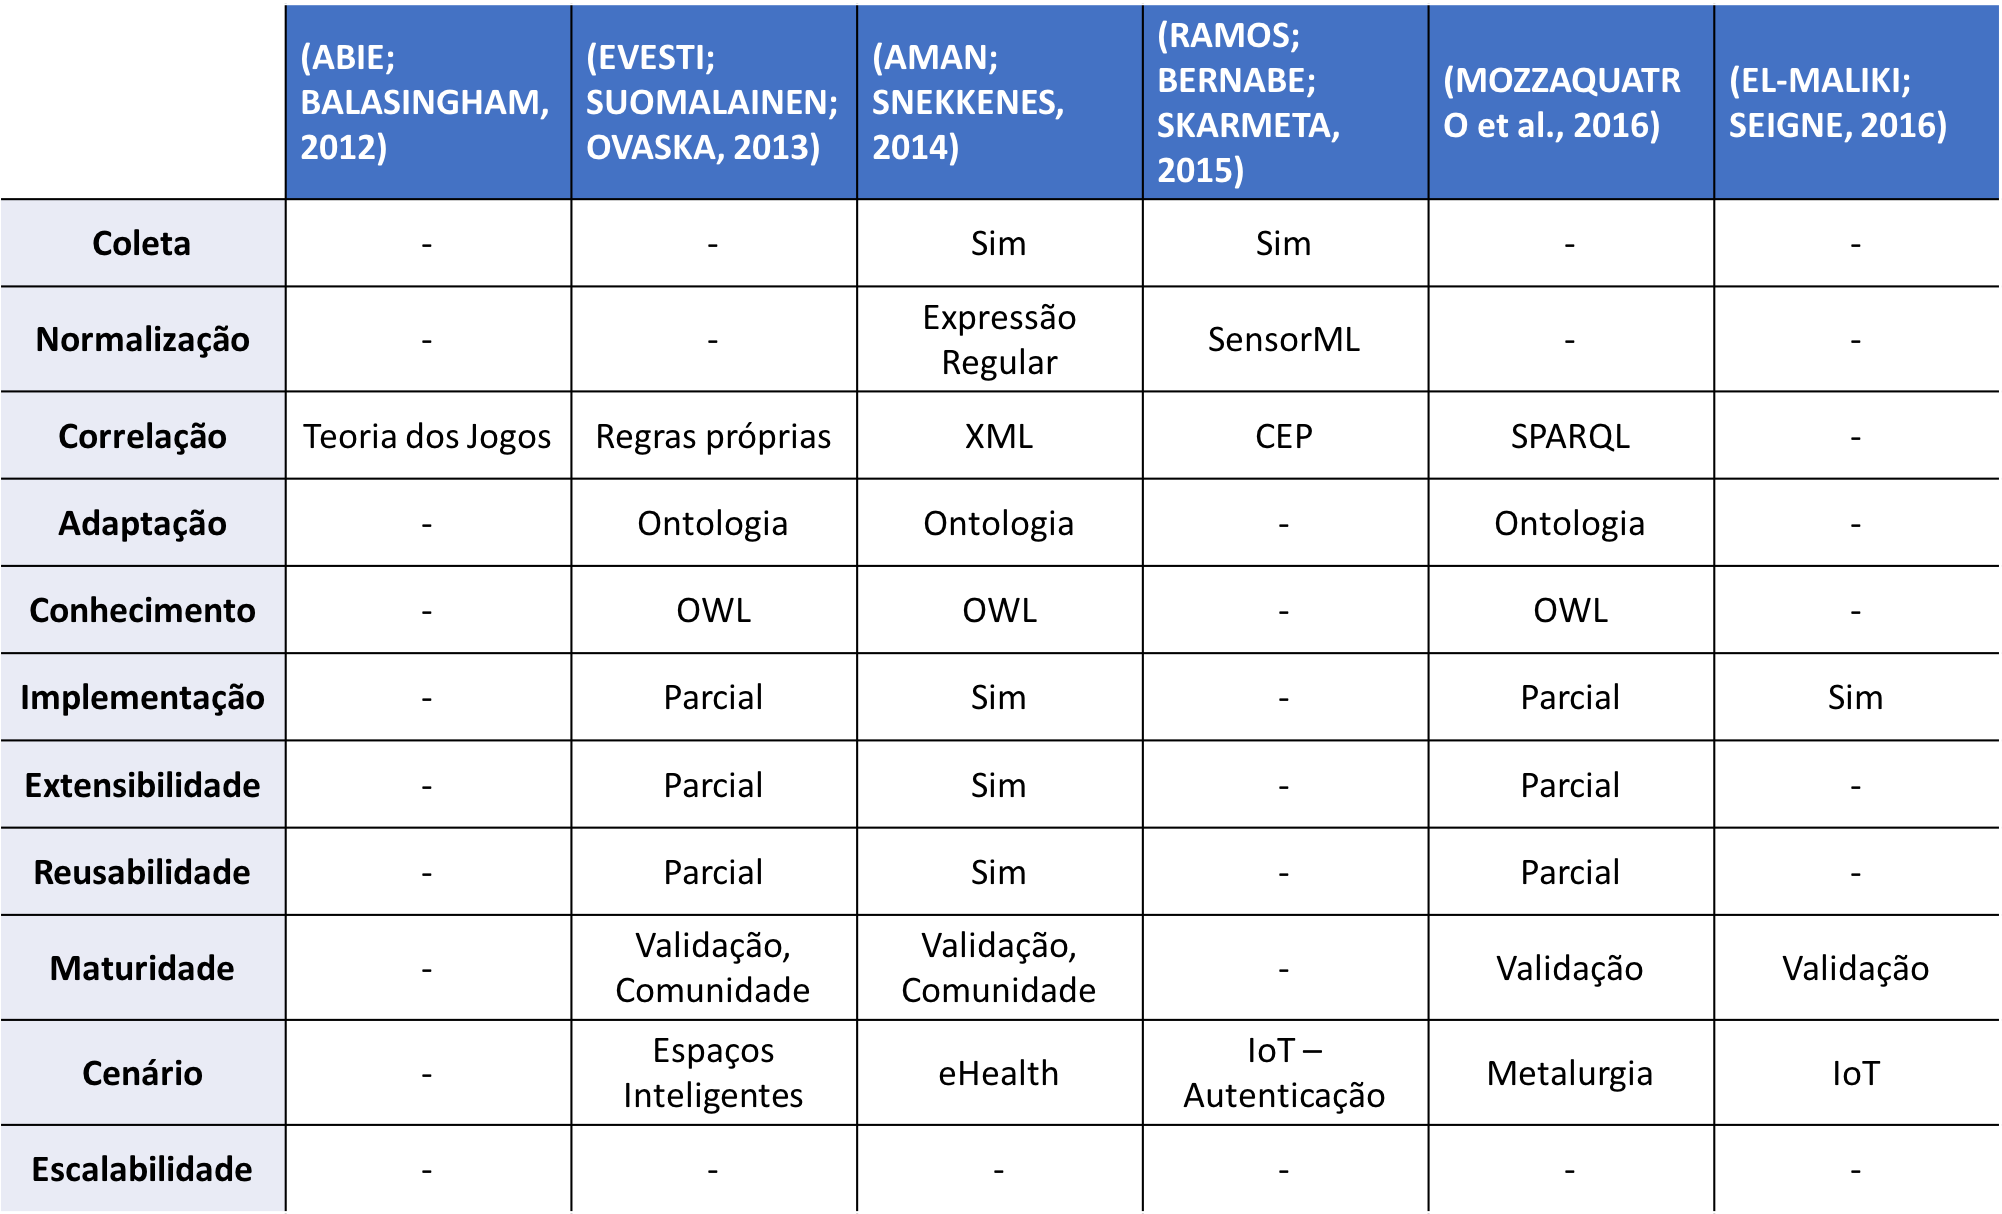
\includegraphics[width=1.0\textwidth]{imagens/comparacao-estado-da-arte.png}
\label{comparacao-estado-da-arte}
\end{table}

Em \cite{evesti13c}, exceto no que tange o emprego da ontologia, os detalhes de implementação identificados por este autor são considerados superficiais e as tecnologias adotadas (como por exemplo, Qt C++) são fortemente dependentes da plataforma empregada. Também não são descritos de forma clara as tecnologias envolvidas para coleta e normalização de eventos. Com isso, apesar do autor Antti Evesti ressaltar a sua abordagem como extensível e reutilizável, para o autor deste trabalho, esta afirmação pode ser aplicada apenas no que tange a ontologia, porém não no seu trabalho de maneira geral.

De forma geral, o quesito maturidade, a maior parte dos trabalhos apresentou cenários para validação da proposta, porém, as tecnologias envolvidas possuem restrição quanto à sua adoção pela comunidade, em especial pela utilização de ontologias, que apesar de ser um tópico importante de pesquisa em desafios de segurança da informação, não é possível afirmar que a sua adoção vem sendo praticada na área.

Percebe-se também que a adoção de ontologias por parte dos trabalhos \cite{evesti13c}, \cite{aman14} e \cite{mozzaquatro16} implica em dificuldades de escalabilidade, sendo em geral uma problemática levantada como limitações em seus trabalhos ou teses derivadas. Além disso, em \cite{aman14}, a tecnologia OSSIM empregada é reconhecida por possuir problemas de estabilidade e escalabilidade \cite{gartner15}, \cite{infosecnirvana14}.

O trabalho \cite{ramos15}, por sua vez, apresenta um modelo genérico, sem detalhar os modelos e tecnologias empregadas. Assim assim, ele destaca alguns dos protocolos geralmente envolvidos para coleta de eventos na IoT, como o \textit{Constrained Application Protocol} (CoAP), \textit{Extensible Messaging and Presence Protocol} (XMPP) ou \textit{Message Queue Telemetry Transport} (MQTT).

El-Maliki apresenta em sua tese \cite{elmaliki14} uma série de testes e simulações realizadas para validação, avaliando em especial a latência decorrente do uso da criptografia e o consumo de energia, os quais evidenciam estratégias de implementação em diferentes cenários da IoT. Apesar disso, o protótipo é fortemente associado ao estudo de caso, não sendo uma abordagem voltada para eventos, consequentemente não possuindo detalhes sobre a coleta de eventos, sua normalização, correlação, armazenamento, bem como estratégia empregada na adaptação. Além disso, não é uma característica a possibilidade de extensão e reuso da proposta.

\section{Considerações do Capítulo}

Este capítulo apresentou os trabalhos identificados como estado da arte em arquiteturas ou \textit{frameworks} genéricos de segurança adaptativa para IoT. O processo para esta análise seguiu o mapeamento sistemático da literatura. Os trabalhos foram descritos em termos do modelo proposto, buscando detalhar as estratégias de concepção e prototipação. Finalmente, foi realizada uma comparação entre os mesmos seguindo características consideradas oportunas considerando as críticas e desafios identificados durante esta revisão. 

%%%%%%%%%%%%%%%%%%%%%%%%%%%%%%%%%%%%%%%%%%%%%%%%%%%%%%%%%%%%%%%%%%%%%%%

\chapter{Considerações Finais}

O presente trabalho buscou apresentar uma revisão conceitual sobre segurança adaptativa para IoT. No decorrer da revisão foi possível perceber os diferentes desafios existentes na IoT que potencializam a segurança da informação enquanto estratégia para viabilização dos inúmeros benefícios decorrentes deste paradigma. 

Com isso, foi encaminhada a necessidade de arquiteturas para segurança adaptativa que promovam a adaptação dinâmica dos mecanismos de segurança de forma que as mudanças aplicadas não prejudiquem a eficiência, flexibilidade, confiabilidade e segurança dos ambientes da IoT. Tendo em vista a natureza ubíqua,
%\AY{ubíqua  - padronizar: ou pervasiva ou ubíqua} - feito
distribuída e dinâmica da IoT, as informações contextuais devem ser um dos principais componentes para conduzir o comportamento dos dispositivos a fim de tornar as decisões de segurança adequadas ao ambiente. 

Para a concepção dessas arquiteturas foi apresentado o ciclo de \textit{feedback} MAPE-K, o qual consiste de um método formal que estabelece as etapas a serem executadas para a adaptação. É importante salientar que para implementar cada umas destas etapas algumas questões devem ser respondidas. Além disso, um sistema adaptativo deve contemplar auto-atributos como: autoconfiguração, auto-otimização, autocura e autoproteção. Não obstante, pesquisas vem sendo desenvolvidas nessa área indicando a ciência de contexto como outro atributo a ser explorado.

Desta forma, a segurança adaptativa baseada em contexto envolve a coleta de informações contextuais tanto do sistema como do meio ambiente, medindo o nível de segurança e as métricas, realizando o processamento dessas informações coletadas e respondendo às mudanças (i) ajustando parâmetros internos, como esquemas de criptografia, protocolos de segurança, políticas de segurança, algoritmos, diferentes mecanismos de autenticação e autorização, alterando a QoS e automatizando a reconfiguração dos mecanismos de proteção e/ou (ii) fazendo mudanças dinâmicas na estrutura do sistema de segurança \cite{habtamu12}.

Atualmente, existem várias abordagens para segurança adaptativa \cite{elkhodary07, yuan12}. No entanto, conforme ressaltado no capítulo sobre o estado da arte, as abordagens existentes se concentram em objetivos de segurança específicos. Percebe-se também a falta no tratamento total do ciclo de \textit{feedback}, ou seja, as abordagens não definem todo o ciclo MAPE. Além disso, Yuan et al. observa que as arquiteturas genéricas não detalham os métodos usados em cada componente, o que dificulta a reutilização e extensibilidade das abordagens propostas. Com o mapeamento sistemático realizado neste trabalho, foi possível identificar que apesar dos avanços nas pesquisas em segurança adaptativa em diferentes frentes, os desafios mencionados continuam em aberto, existindo ainda poucas abordagens genéricas que detalhem a sua concepção, prototipação e estratégias de avaliação.

%\section{Perspectiva de Investigação}

%\section{Trabalhos Futuros}

%%%%%%%%%%%%%%%%%%%%%%%%%%%%%%%%%%%%%%%%%%%%%%%%%%%%%%%%%%%%%%%%%%%%%%%
\bibliography{bibliografia}
\bibliographystyle{abnt}

\end{document}